 \mychapter{Moviments en el pla i l'espai}{Moviments en el pla i l'espai}{\begin{center}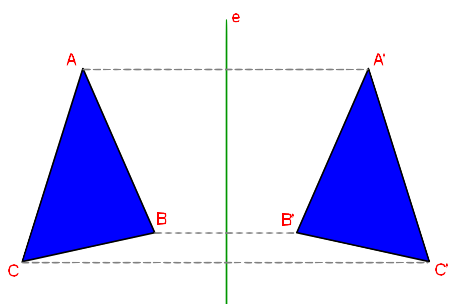
\includegraphics[width=1.1\textwidth]{img-10/especular} \footnotesize Simetria especular. És la imatge que forma un mirall.\end{center}}{chap:moviments}
 

\begin{iniaval}
	
	Observa les imatges. Descriu en cada cas com s'han obtingut els diferents personatges a partir de l'inicial.
	
	\begin{center}
		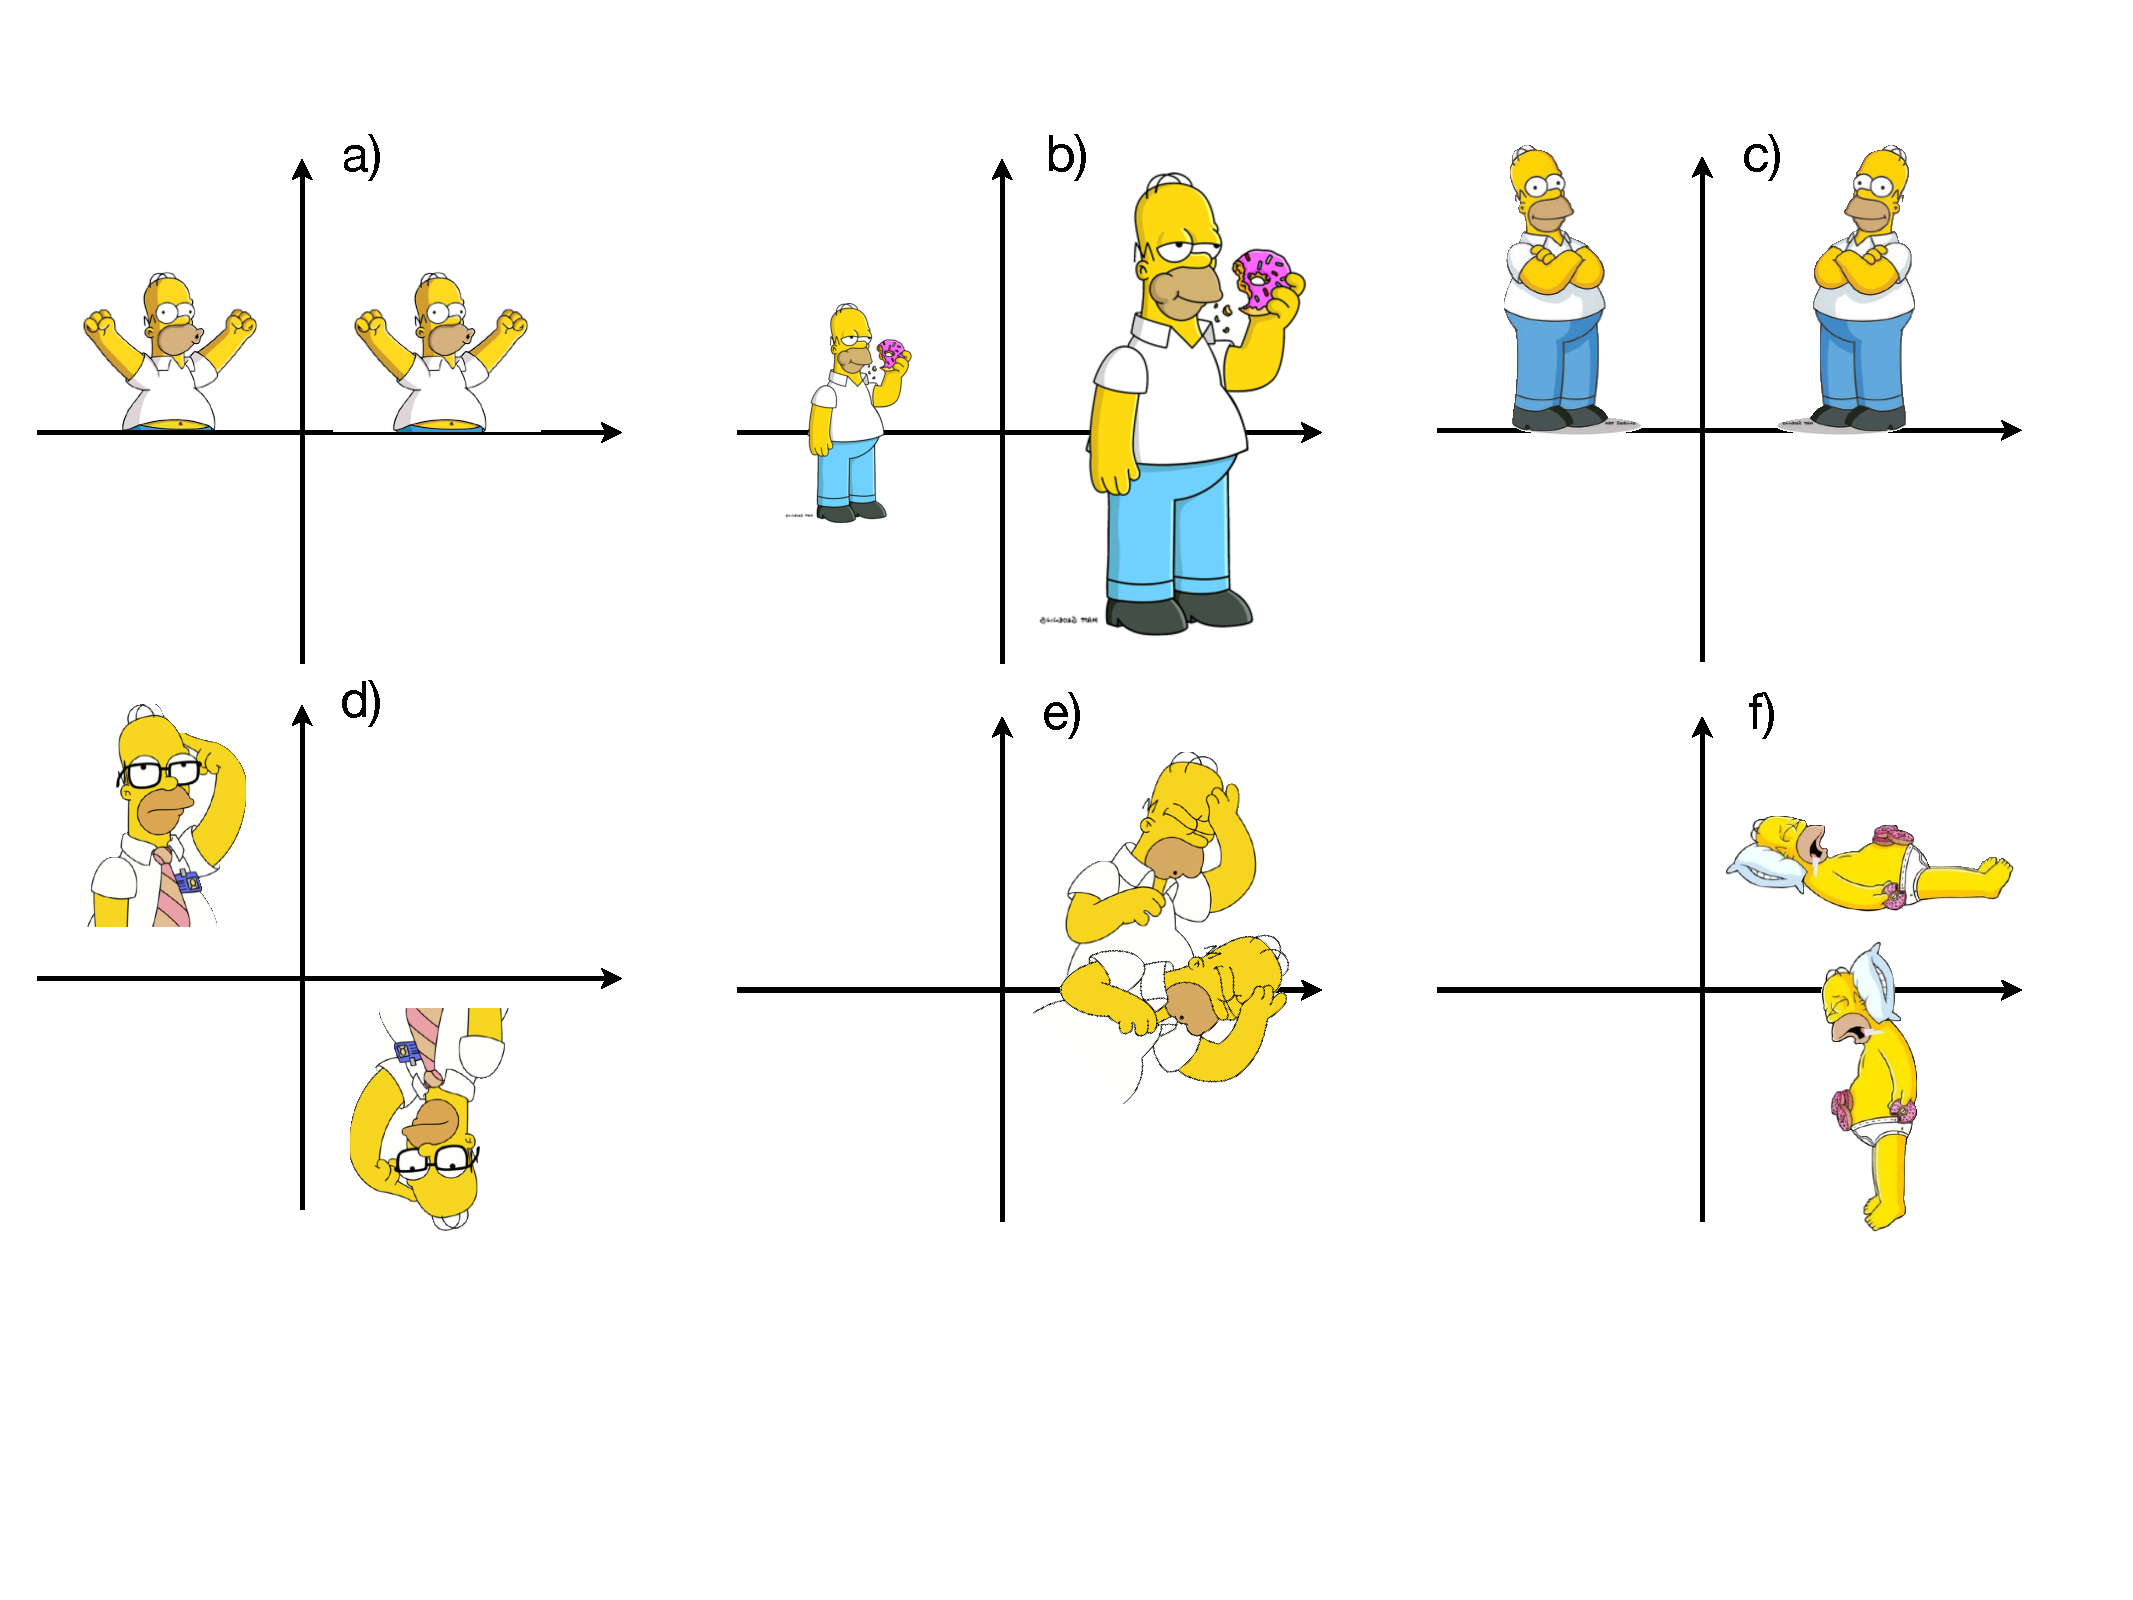
\includegraphics[width=0.9\textwidth]{img-10/iniaval}
	\end{center}

	Sabries col·locar el nom de cada transformació? 
	
	\begin{center}
		 \textbf{ Homotècia, Simetria central, Translació, Simetria axial, Gir. }
	\end{center}
	\addanswersline[cols=1]{Avaluació inicial}{0}{[Translació, Homotècia, Simetria axial, Simetria central, Rotació, Rotació de $270^\circ$ + simetria axial]}
\end{iniaval}

\section{Transformacions geomètriques}


\begin{theorybox}
	Una \textbf{transformació geomètrica} converteix cada punt del pla en un altre punt. Una figura es transforma en una altra figura.
	
	Les transformacions que estudiarem són: La translació, l'homotècia, la simetria axial i central i els girs o rotacions.
\end{theorybox}

\begin{mylist}
\exer  En el teu quadern dibuixa un triangle. Calca-ho i copia la figura calcada de nou en el teu quadern. Mesura tots els costats de les figures homòlogues. Mesuren el mateix? Mesura tots els seus angles. Mesuren el mateix?

\answers{Gràfica:\par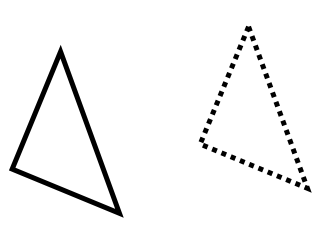
\includegraphics[width=0.34\textwidth]{img-sol/t10-1}\par Hem fet una translació: Tots els costats i tots els angles mesuren el mateix que el triangle original. }

\exer  Dibuixa en el teu quadern una lletra \textbf{B} i fes un disseny amb ella, traslladant-la, girant-la o dibuixant lletres \textbf{B} simètriques.

\answers{Gràfica:\par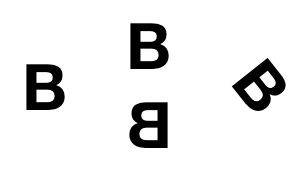
\includegraphics[width=0.34\textwidth]{img-sol/t10-2}}

\exer  En el teu quadern dibuixa una lletra \textbf{b} minúscula, i a continuació una altra lletra \textbf{b} minúscula el doble de gran. Com són les seves longituds i els seus angles? És una semblança?

\answers{Els costats són el doble de grans i els angles són iguals. És una semblança de raó 2:\par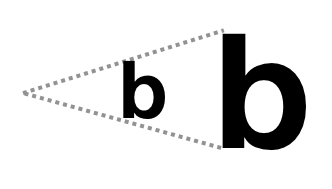
\includegraphics[width=0.4\textwidth]{img-sol/t10-3}}

\exer  Dibuixa ara una lletra \textbf{d} minúscula. És semblant a la lletra \textbf{b} anterior?

\answers{La lletra \textbf{d} minúscula és una simetria especular de la \textbf{b} anterior.}

\exer  En el teu quadern marca una trama formada per quadrats de dos quadradets de costat. En un quadradet dibuixa una taca, una poligonal, una línia corba{\dots} Dibuixa la simètrica prenent com a eix de simetria un costat del quadrat. Dibuixa la figura simètrica del conjunt obtingut prenent com a eixos sempre els costats de la trama inicial. Acoloreix la figura obtinguda. Trasllada-la horitzontal i verticalment.

\answers{Gràfica:\par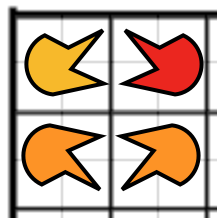
\includegraphics[width=0.34\textwidth]{img-sol/t10-5}}

\end{mylist}
 
\section{Translacions}
\vspace{-0.25cm}
\subsection{Vectors}
\vspace{-0.25cm}
\begin{theorybox}
	\begin{minipage}{0.6\textwidth}
			Donats dos punts $A$ i $B$, definim el vector fix $\overrightarrow{AB}$ com el segment orientat que els uneix. $A$ és el punt d'\textbf{origen} i $B$ és l'\textbf{extrem} del vector.
		
		Per calcular el vector restam les components dels punts. 
		
		Per exemple, si $A(-1, 2)$ i $B(3, -1)$, $\overrightarrow{AB}=B-A =(3, -1)-(-1, 2)=(4, -2)$. Això significa que per anar de $A$ cap a $B$ avançam 4 unitats en $x$ i baixam 2 unitats en $y$.
	\end{minipage}
\begin{minipage}{0.4\textwidth}
	\centering
	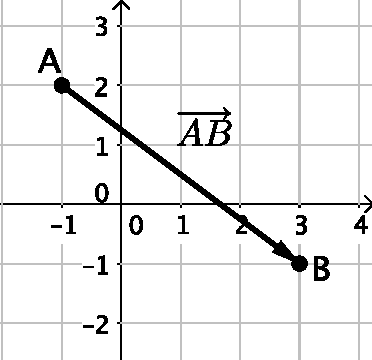
\includegraphics[width=0.7\textwidth]{img-10/vector-example}
\end{minipage}

\end{theorybox}

\begin{mylist}
\exer  Dibuixa en el teu quadern els punts de coordenades \textit{A}(  $-$5, 2), \textit{B} ($-$1, 6) i \textit{C} (2, $-$3). Troba les coordenades dels vectors fixos $\overrightarrow{AB}$, $\overrightarrow{AC}$, $\overrightarrow{BC}$, $\overrightarrow{CA}$ i $\overrightarrow{CB}$. Comprova en el teu dibuix que aquestes són les seves coordenades.
\answers{Gràfica:\par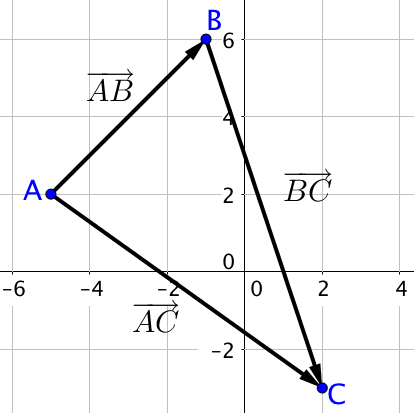
\includegraphics[width=0.34\textwidth]{img-sol/t10-6}\par
$\overrightarrow{AB}=B-A=(4, 4)$, $\overrightarrow{AC}=C-A=(7, -5)$, $\overrightarrow{BC}=C-B=(3,-9)$, $\overrightarrow{CA}=A-C=(-7,5)$ i $\overrightarrow{CB}=B-C=(-3,9)$}
 
\exer  El vector fix $\overrightarrow{AB}$ té de coordenades (4, 2), calcula les coordenades del seu origen \textit{A} sabent que les coordenades del seu extrem \textit{B} són ($-$1, 1). Representa-ho gràficament.
\answers{Gràfica:\par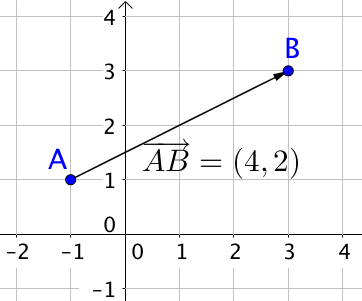
\includegraphics[width=0.34\textwidth]{img-sol/t10-7}\par
	$\overrightarrow{AB}=B-A$ $\rightarrow$, $(4,2)=B-(-1,1)$ del qual aïllam $B=(4,2)+(-1,1)=(3,3)$.} 

\vspace{-1.8cm}
\exer \begin{minipage}[t]{0.5\textwidth}
	Escriu les coordenades dels vectors fixos de la figura i indica quins són representants d'un mateix vector lliure.
\end{minipage}
\begin{minipage}{0.5\textwidth}
	\centering
	\vspace{1.5cm}
	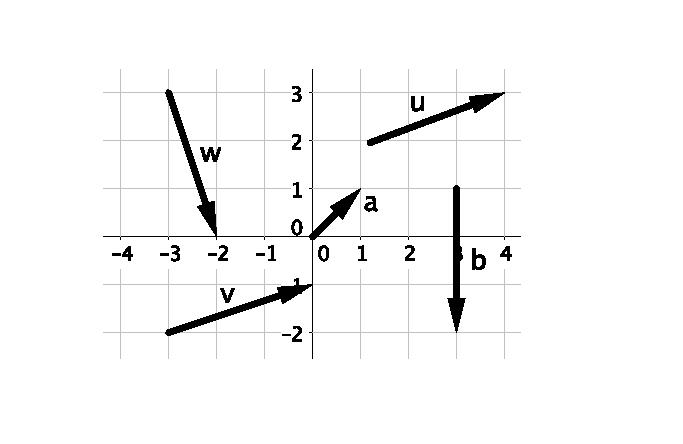
\includegraphics[width=0.6\textwidth]{img-10/vectors}
\end{minipage}
\answers{$\vec a =(1,1)$; $\vec b=(0,-3)$; $\vec u=(3,1)$; $\vec v=(3,1)$; $\vec w=(1,-3)$. Els vectors $\vec u$ i $\vec v$ són representats del mateix vector lliure.}


 \exer  Les coordenades de A són (2, 3) i les del vector fix $\overrightarrow{AB}$ són (4, $-$2). Calcula les coordenades del punt \textit{B}. Representa-ho gràficament.
 \answers{Gràfica:\par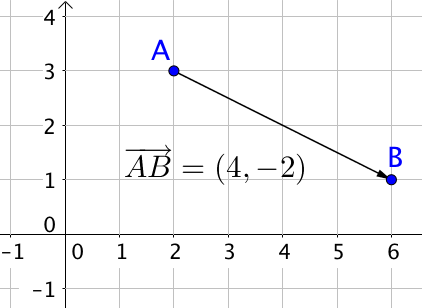
\includegraphics[width=0.34\textwidth]{img-sol/t10-9}\par
 	$\overrightarrow{AB}=B-A$ $\rightarrow$, $(4,-2)=B-(2,3)$ del qual aïllam $B=(4,-2)+(2,3)=(6,1)$.} 

\exer  Dibuixa en el teu quadern quatre vectors equipol·lents al vector fix amb origen en  $A( -3, 4)$ i extrem $B(5, 0)$, amb orígens en els punts \textit{C} (0, 3), \textit{D} (5, 2), \textit{E}($-$4, 0) i \linebreak \textit{F} ($-$2, $-$5). 

\answers{Solució gràfica:\par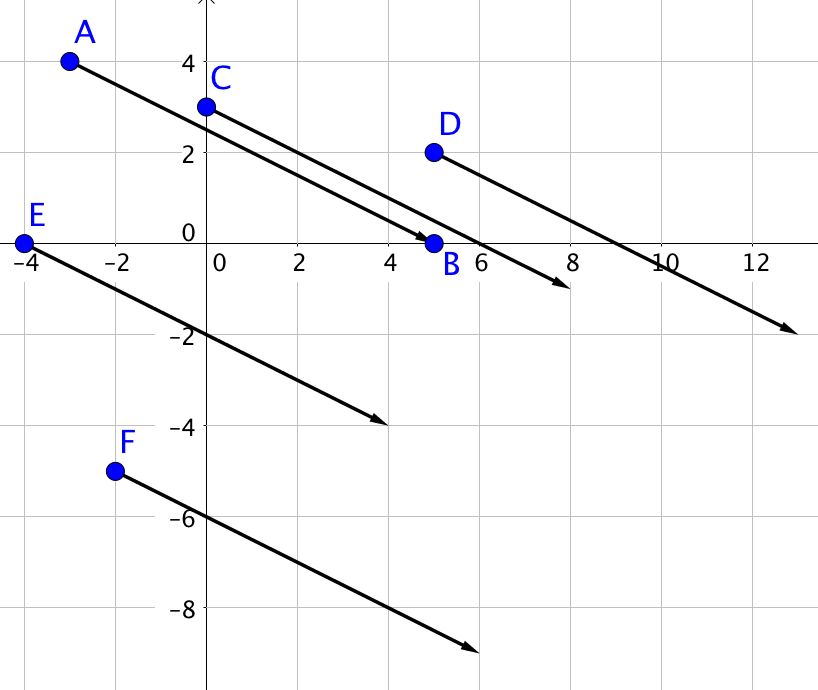
\includegraphics[width=0.4\textwidth]{img-sol/t10-equipolent}} 


\exer  Dibuixa en el teu quadern els punts \textit{A}( $-$2, 2), \textit{B} ($-$3, 0), \textit{C} (2, 4), \textit{D} (6, 2), \textit{E} (2, 0), \linebreak \textit{F} (6, $-$2) i \textit{G }(2, $-$4). Amb els vectors fixos d'origen i extrem en aquests punts, indica quins d'ells són equipol·lents.

\exer  Amb els punts de l'exercici anterior, calcula les coordenades dels vectors fixos $\overrightarrow{DE}$ i $\overrightarrow{FG}$. Com són? Són dos representants d'un mateix vector lliure?

\answers{$\overrightarrow{DE}=D-E=(-4,-2)$ i $\overrightarrow{FG}=G-F=(-4,-2)$ són equipol·lents. Sí. Són representants d'un mateix vector lliure.}

\exer  Dibuixa en el teu quadern un sistema de referència cartesià i assenyala en ell els punts de coordenades: \textit{A} (4, 5), \textit{B}~(-5,~6) i \textit{C} (2, --5).


\begin{tasks}
	\task  Anomena $\vec u$ al vector fix $\overrightarrow{AB}$ i indica els seus components.
	\task  Anomena $\vec v$ al vector fix $\overrightarrow{BC}$ i indica els seus components.
	\task  Calcula les components del vector $\vec w$= $\vec u$ + $\vec v$.
	\task  Representa en el teu quadern els vectors lliures $\vec u$ i $\vec v$ amb origen en l'origen de coordenades i representa també al vector suma $\vec w$. Observa que està sobre la diagonal del paral·lelogram construït sobre $\vec u$ i $\vec v$.
\end{tasks}

\answers[cols=1]{[$\vec u = (-9,-11)$, $\vec v=(7,-11)$, $\vec w=(-2,-10)$]}

\end{mylist}

\begin{theorybox}[Operacions amb vectors lliures]
Donats els vectors $\vec v =(-2, 3)$ i $\vec u=(5, 4)$ podem realitzar les següents operacions
\begin{itemize}
	\item  Multiplicar un vector per un número:  $5 \vec v = 5 (-2, 3)=(-10, 15)$ 
	\item Sumar dos vectors:  $\vec v + \vec u = (-2, 3) + (5, 4) = (3, 7)$
	\item Restar dos vectors:  $\vec v - \vec u = (-2, 3) - (5, 4) = (-7, -1)$
	\item Fer una combinació lineal:  $3\vec v - 2\vec u = 3(-2, 3) - 2(5, 4) = (-6, 9) - (10, 8) = (-16, 1)$ 
\end{itemize}
\end{theorybox}

\begin{mylist}


\exer[1]  Efectua les següents operacions amb els vectors $\vec u$\textit{ }= (--5, 6), $\vec v$= (4, --7) i $\vec w$ = (3, 4):

\begin{tasks}(3)
	\task  2$\vec u$ -- ($\vec v$+ $\vec w$)   
	\task  3$\vec w$ -- 2$\vec u$ + $\vec v$   
	\task   2($\vec u$ + $\vec v$) -- 3$\vec w$
\end{tasks}
\answers[cols=1]{[$(-17,15)$, $(23,-7)$, $(-11,-14)$]}

\exer  Dibuixa en el teu quadern el punt \textit{A} (1, 2), dibuixa ara el vector $\vec u$ = (2, 3) amb origen en A , i el vector $\vec v$ = (4, $-$1) també amb origen en A. Calcula les coordenades del vector suma $\vec u$+ $\vec v$, i dibuixa-ho amb origen en A . El resultat coincideix amb el que has obtingut gràficament? Observa que el vector suma és la diagonal d'un paral·lelogram construït sobre $\vec u$ i $\vec v$.

\answers{El vector $\vec u + \vec v = (6,2)$. Si el dibuixam en origen el punt $A(1,2)$, aleshores el vector suma té extrem en el punt $B(7,4)$}

\exer  Efectua les següents operacions amb vectors:

\begin{tasks}(2)
	\task   (5, --9) -- [(6, 3) + (--4, --6)]   
	\task    $3\cdot \left(\frac{1}{3} ,\; -\frac{5}{6} \right)+\frac{1}{2} \cdot (4,\; 8)$      
	\task  5·[(--1, 0) -- (--2, 3)] + (--3)·[(4, --2)]   
	\task  9'3·(2, 6) + (3'7, 5'2)
\end{tasks}

 \answers{[$(3,-6)$, $(3,\frac{3}{2})$, $(65,-99)$, $(22.3,61)$]}

\end{mylist}

\subsection{Translacions}

\begin{theorybox}
	
	 
 	\begin{minipage}{0.5\textwidth}
		Una translació de vector $\vec t$ és una transformació que fa correspondre a cada punt $P$ de la figura inicial el nou punt $P'=P+\vec t$.
	\end{minipage}
	\begin{minipage}{0.5\textwidth}
		\centering
	 
		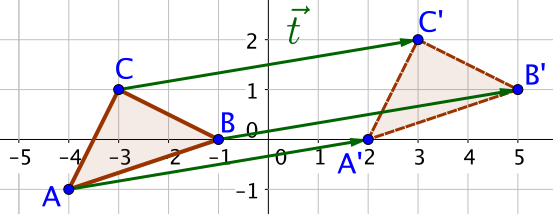
\includegraphics[width=0.95\textwidth]{img-10/translacio}
	\end{minipage}
	
	Si a una figura li feim una translació $\vec t_1$ seguida d'una translació $t_2$, el resultat és equivalent a fer una única translació de vector $\vec t = \vec t_1 + \vec t_2$.
	
	
\end{theorybox}

\begin{mylist}
	
	
	
	
	\exer Dibuixa en el teu quadern una figura i utilitza escaire i cartabó per traslladar-la 5 centímetres cap a la dreta.
	
	\exer  Dibuixa en el teu quadern una figura. (Si no se t'ocorre cap altra, dibuixa la lletra G). Col·loca damunt un paper vegetal i calca-la. Desplaça en línia recta el paper vegetal i torna a calcar la figura. Les dues figures que has obtingut, tenen totes les seves mesures, tant longituds com a angles, iguals? Traça les rectes que uneixen parells de punts corresponents, com són aquestes rectes? Quina trajectòria han seguit els punts en el desplaçament?
	
	\answers{Les dues figures tenen totes les seves longituds i angles iguals. Aquestes rectes són
		paral·leles. Han seguit un vector lliure.}
	
	\exer[1]  Trasllada una figura (per exemple una lletra L) mitjançant el vector \linebreak $\vec t_1= (-4, 5)$ i repeteix el procés amb la figura traslladada emprant el vector  $\vec t_2= (3, -6)$. Quin moviment utilitzes per anar de la primera figura a l'última? És una translació? Quin és el seu vector?
	\answers{És una translació de vector $\vec t_1 + \vec t_2 = (-1,-1)$}
	
	\exer  Utilitza paper quadriculat i dibuixa en el teu quadern una lletra F de 2 quadradets d'alt i 1 quadradet d'ample. A aplica-li una translació de vector (2, 5). 
	
	\exer  Dibuixa en el teu quadern uns eixos cartesians i el triangle de vèrtexs \textit{A} (3, 1), \linebreak \textit{B} (3, 3) i \textit{C} (1, 3). Aplica-li la translació de vector (4, 2): 4 unitats a la dreta i 2 unitats cap amunt. Quines són les coordenades dels punts traslladats \textit{A'}, \textit{B'} i \textit{C'}?
	
	\answers{$A’ = (7, 3)$; $B’ = (7, 5)$; $C’ = (5, 5)$}
	

%\exer  Amb ajuda de paper quadriculat transforma mitjançant una translació una recta, una circumferència, un segment, un triangle, dues rectes paral·leles i dues rectes perpendiculars. En què es transformen? Analitza els resultats.

\exer Representa gràficament la recta $r: \, y=4x-3$ i el vector $\vec t(1,4)$. Comprova que si traslladam la recta $r$ segons el vector $\vec t$ obtenim la mateixa recta. 
 
 	\answers{Gràfica:\par 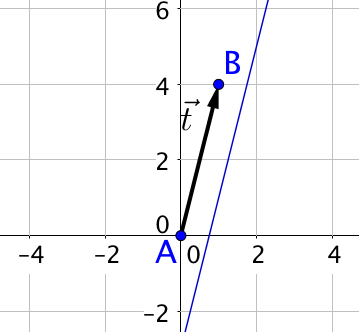
\includegraphics[width=0.35\textwidth]{img-sol/t10-23}}
 	
\end{mylist}
 

\pagebreak

\section{Girs o rotacions}

\begin{theorybox}[Girs]
	 
	\begin{minipage}{0.5\textwidth}
		Un gir de centre $O$ i angle $\alpha$ és una transformació que fa correspondre a cada punt $P$ de la figura inicial el nou punt $P'$, tal que:
		\[  \overline{OP}=\overline{OP'}  \text{  i  }  \widehat{POP'}=\alpha \]
		
		Quan l'angle és positiu, el gir és en sentit antihorari (contrari a les agulles del rellotge).
	\end{minipage}
	\begin{minipage}{0.5\textwidth}
		\centering
		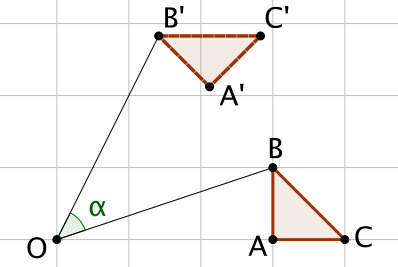
\includegraphics[width=0.985\textwidth]{img-10/rotacio}
		
	\end{minipage}
	
	
\end{theorybox}

\begin{mylist}
\exer  Dibuixa en el teu quadern un punt \textit{O} i un altre punt diferent \textit{A}. Gira al punt \textit{A} amb centre en  O un angle de 30º en sentit positiu i denomina \textit{A'} el punt girat.

\exer  Dibuixa en el teu quadern un punt \textit{O} i dos segments, un \textit{OA} que passa per\textit{ }O , i un altre \textit{BC} que no passa per O . Dibuixa els segments girats \textit{OA'} i \textit{B'C'} del gir de centre \textit{O} i angle 60º.

\exer[1]  Dibuixa en el teu quadern el triangle de vèrtexs \textit{A} (4, 2), \textit{B} (3, $-$2) i \textit{C} (5, 0). Dibuixa el triangle que s'obté en girar-ho amb centre en l'origen de coordenades un angle de 90º en sentit positiu. Quines són les coordenades dels vèrtexs \textit{A'}, \textit{B'} i \textit{C'} del triangle girat?
\answers{\textit{A'} (2, 4), \textit{B'} ($-$2, 3) i \textit{C'} (0, 5)}

\exer  Amb ajuda de paper quadriculat, transforma mitjançant un gir, una recta, una circumferència, un segment, un triangle, dues rectes paral·leles i dues rectes perpendiculars. En què es transformen? Analitza els resultats.

\answers{	Mitjançant el gir la recta es transforma en una recta, la
	circumferència, el segment i el triangle en una circumferència, un
	segment i un triangle igual, respectivament. Dues rectes paral·leles en dos
	rectes paral·leles, i dues rectes perpendiculars, en dues rectes
	perpendiculars.}


\exer  Dibuixa en el teu quadern dos punts qualssevol \textit{P} i \textit{P'}. Troba el seu centre de simetria.

\exer[1]  Què ocorre en aplicar un gir de 60º a una figura? Hi ha rectes invariants? I en un gir de 180º? Les rectes que passen pel centre de gir, en quines rectes es transformen? I amb un gir de 0º? I amb un gir de 360º?
\answers{
	Un gir de $60^\circ$ no deixa cap recta invariant. Un gir de $180^\circ$ deixa invariants les rectes que passen del centre de gir. Les rotacions de $0^\circ$ i $360^\circ$ són la identitat, deixen la figura original. 
 }

\exer  Dibuixa un triangle \textit{ABC} i el seu simètric \textit{A'B'C'} respecte un punt \textit{O}. Com són els seus costats? Són iguals? I els seus angles? Es manté el sentit dels angles? Comprova com és l'angle \textit{ABC} i l'angle \textit{A'B'C'}. És un moviment directe?

\answers{Recorda que la simetria central en el pla és un gir de 180$^\circ$, llavors és un moviment
	directe. Els costats i els angles d'un triangle i el seu girat 180 són iguals, i amb el mateix sentit.}

\exer  Anem a analitzar les lletres majúscules. Indica quines de les següents lletres no tenen simetria central i quines si la tenen, indicant llavors el seu centre de simetria: B, H, N, O, P, S, T, X, Z. Recorda, cerques un punt tal que la simetria central de centre en aquest punt deixi invariant a la lletra.

 \answers{No tenen simetria central: B, P, T. Si la tenen: H, N, O, S, X, Z.}

\exer  Mitjançant un gir en l'espai, en què es transforma un pla? I una esfera? I un con? I dos plans paral·lels? I dos plans ortogonals? Analitza els resultats.

\answers{El pla es transforma en un pla, una esfera en una esfera igual, un con en un altre con igual, els plans
	paral·lels es transformen en plans paral·lels i els ortogonals en plans ortogonals.
}
\end{mylist}
 

\pagebreak
\section{Simetries}

\begin{theorybox}
	S'anomena una \textbf{simetria d'eix $e$} a una transformació que fa correspondre a cada punt $P$ un altre punt $P'$ de tal forma que la recta $e$ és la mediatriu del segment $\overline{PP'}$
	
	S'anomena una \textbf{simetria central} a una transformació que fa correspondre a cada punt $P$ un altre punt $P'$ de tal forma que l'origen de coordenades $O(0,0)$ és el punt mitjà del segment $\overline{PP'}$. Aquesta simetria equival a un gir de 180${}^\circ$ respecte l'origen.
	
	\begin{center}
		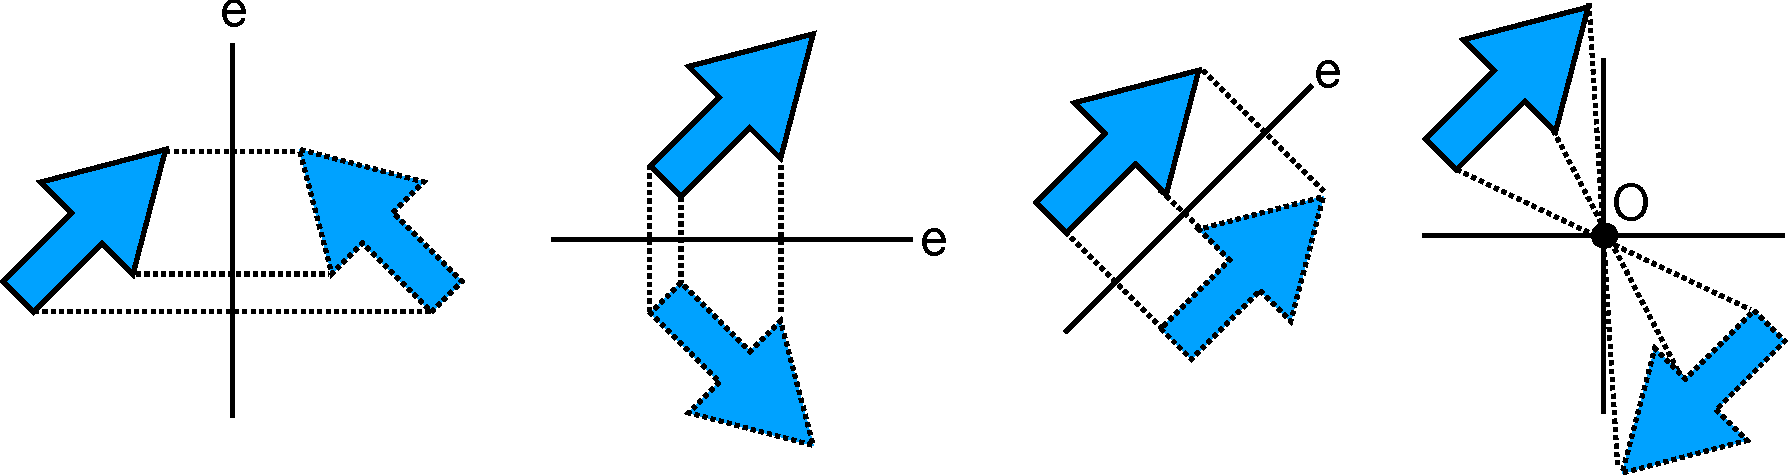
\includegraphics[width=\textwidth]{img-10/simetries}
			\footnotesize
		Diferent tipus de simetries: D'eix vertical, eix horitzontal, eix oblic i simetria central.
	\end{center}
\end{theorybox}

\begin{mylist}

\exer  Dibuixa en el teu quadern un eix \textit{r} de simetria oblic, i un punt P . Dibuixa el punt P' simètric respecte de r . Comprova que la recta \textit{r} és la mediatriu del segment \textit{PP'.} (\textit{Recorda}: La mediatriu d'un segment és la perpendicular pel punt mitjà).

\answers{A forma d'exemple:\par 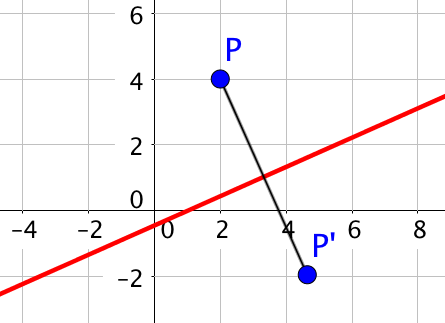
\includegraphics[width=0.35\textwidth]{img-sol/t10-33}}

\exer  Dibuixa en el teu quadern dos punts qualssevol \textit{P} i \textit{P'}. Dibuixa l'eix de simetria \textit{r} respecte al que són simètrics. 

\answers{L'eix de simetria és la mediatriu del segment $\overline{PP'}$}

\exer  Dibuixa en paper quadriculat una lletra \textbf{L} i un eix de simetria vertical. Dibuixa una \textbf{L} simètrica respecte a aquest eix. Calca una d'elles, i mou el paper de calc per intentar fer-les coincidir. Nota que és impossible; perquè la simetria és un moviment invers. 


\exer  Dibuixa en el teu quadern una figura. Dibuixa un eix de simetria oblic i dibuixa la figura simètrica.
 
\answers{A forma d'exemple:\par 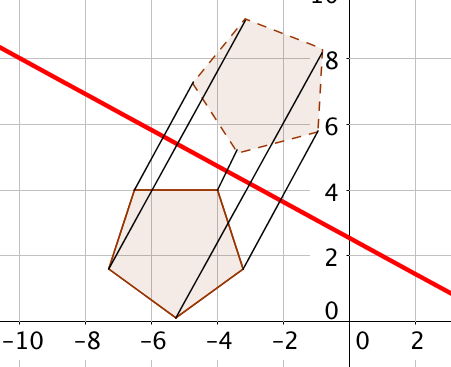
\includegraphics[width=0.35\textwidth]{img-sol/t10-36}}

\exer[1]  Troba les coordenades dels vèrtexs del triangle simètric respecte de l'eix d'ordenades $OY$ del triangle $A(3, -4)$, $B(5, 6)$ i $C(-4, 5)$. Repeteix per l'eix d'abscisses.
\answers{i)  $A'(-3,-4)$, $B'(-5,6)$ i $C'(4,5)$;\par  ii)  $A'(3,4)$, $B'(5,-6)$ i $C'(-4,-5)$}

\answers{Eix d'ordenades: $A’ ( 3,  4)$, $B’ ( 5, 6)$, $C’ (4, 5)$;\par Eix d'abscisses: $A’’ (3, 4)$, $B’’ (5,  6)$, $C’’ ( 4,  5)$}

\vspace{-2.5cm}
\exer \begin{minipage}[t]{0.6\textwidth}
	Reprodueix en el teu quadern la figura de l'ocell P del marge. 
	
	\begin{tasks}
		\task  Dibuixa l'ocell P' simètric respecte a l'eix d'ordenades.
		\task  Dibuixa l'ocell P'' simètric respecte a l'eix d'abscisses. 
		\task  Existeix alguna simetria axial que transformi P' en P''? Existeix alguna simetria central que transformi P' en P''?
	\end{tasks}
\end{minipage}
\begin{minipage}{0.4\textwidth}
	\centering
	\vspace{2.5cm}
	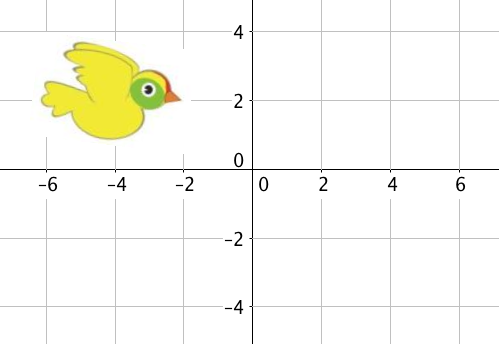
\includegraphics[width=0.8\textwidth]{img-10/ocell}
\end{minipage}

\begin{tasks}[resume=true]
	\task  Si el bec de l'ocell P tingués unes coordenades ($-2$, $2$), quines coordenades tindria el bec de l'ocell P'? I el de l'ocell P''?
\end{tasks}
 
 \answers{a, b) Solució gràfica:\par 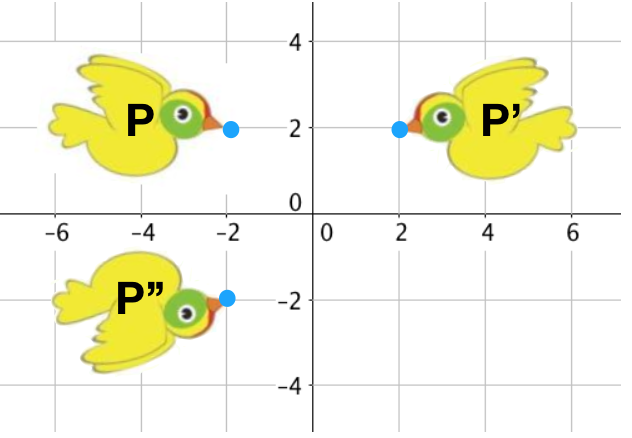
\includegraphics[width=0.35\textwidth]{img-sol/t10-38}\par c) No existeix cap simetria aixal. Sí. Una simetria central en centre l'origen. \par d) $P'(2,2)$ i $P''(-2,-2)$}
 
\exer \mental Indica quines de les lletres majúscules són simètriques, i si ho són, indica si els seus eixos de simetria són horitzontals o verticals: A, B, D, F, K, M, N, R, T, O, V, W.

\answers{Eix de simetria horitzontal: B, D. Eix de simetria vertical: A, M, T, U, V, W.}

\exer  Amb ajuda de paper quadriculat, transforma mitjançant una simetria, una recta, una circumferència, un segment, un triangle, dues rectes paral·leles i dues rectes perpendiculars. En què es transformen? Analitza la resposta.

\answers{Mitjançant una simetria la recta es transforma en una recta, la circumferència, el
	segment i el triangle en una circumferència, un segment i un triangle igual, respectivament. dos
	rectes paral·leles a dues rectes paral·leles, i dues rectes perpendiculars, en dues rectes perpendiculars.}

\exer  Dibuixa un rectangle \textit{ABCD}. Dibuixa l'eix de simetria que transforma \textit{AB} en \textit{CD}, i l'eix de simetria que transforma \textit{AD} en \textit{BC}.

\answers{ El rectangle té dos eixos de simetria, les mediatrius dels segments AB i BC}

\exer  Dibuixa un hexàgon regular i dibuixa els seus eixos de simetria. Quants té? Fes el mateix per un pentàgon regular.

\answers{ L'hexàgon té 6 eixos de simetria, 3 van de vèrtex a vèrtex oposat, i 3 van de
	centre de costat a centre de costat oposat.\par El pentàgon té 5 eixos de simetria, que van de vèrtex al centre del costat oposat.}

\exer  Dibuixa en el teu quadern dos eixos de simetria paral·lels i una lletra F. Dibuixa la composició d'ambdues simetries a aquesta lletra, comprovant que la composició d'elles és una translació i determina el vector de translació.

\answers{El vector de translació és perpendicular a la direcció de les rectes, de sentit de la
	primera recta a la segona i de mòdul, el doble de la distància entre les rectes.}

\exer  Dibuixa en el teu quadern dos eixos de simetria secants i una lletra F. Dibuixa la composició d'ambdues simetries a aquesta lletra, comprovant que la composició d'elles és un gir i determina el centre i l'angle de gir.

\answers{El centre de gir és el punt d'intersecció de les rectes, i l'angle de gir té
	d'amplitud el doble de l'angle que formen les rectes i de sentit, de la primera recta a la segona.}

\exer  Si apliquem una simetria a una figura, quina transformació hem d'aplicar-li per obtenir la figura inicial?

\answers{La mateixa simetria. Les simetries són involutives, és a dir $S \circ S=$Identitat.}
 
\exer  La composició de dues simetries planes d'eixos secants és un gir. Com han de ser els eixos perquè sigui un gir de $180^\circ$ (o una simetria central)?

\answers{Cal que els eixos siguin ortogonals}

\exer   Escriu cinc objectes que estiguin al teu al voltant que siguin simètrics i indica el seu pla de simetria. Mira a l'aula i busca simetries. Són simètriques les cadires, el llum, la finestra, les taules...? Quin és el seu pla de simetria?

\answers{ Per exemple: la meva cadira, la taula, el meu ordinador, el llum, un llapis.}
 
\exer  Defineix els plans de simetria i els eixos de rotació de les següents figures:
\begin{tasks}
	\task  Un prisma recte de base quadrada. I si és oblic?
	\task  Una piràmide recta de base quadrada.
	\task  Si el prisma i la piràmide són rectes, però les seves bases són rectangles, quines simetries es mantenen?
\end{tasks}

\answers[cols=1]{[Té 5 plans de simetria; 2 passen per 4 vèrtexs i 2 arestes laterals; 2
	passen pels punts mitjans de 4 arestes de la base; 1 passa pels punts
	mitjans de les arestes laterals. Té un eix de rotació de 90$^\circ$, 180$^\circ$ i 270$^\circ$ que
	va de centre de la base quadrada a centre de l'altra base. \par Si és unn prisma oblic; no en té cap.,
	%%
	Piràmide de base
	quadrada té 4 plans de simetria;  2 passen per 2 vèrtexs de la base i el vèrtex i els altres 2; pels punts
	mitjans de les arestes de la base i el vèrtex. Té un eix de rotació de 90$^\circ$, 180$^\circ$ i 270$^\circ$ que passa pel vèrtex i el centre de quadrat de la base,
	%%
	Es perden els plans de simetria que passen per dues arestes.
	]}


\exer   Determina els plans de simetria i els eixos de rotació d'aquestes figures:
\begin{tasks}
	\task  Un prisma recte la base del qual és un triangle equilàter.
	\task  Una piràmide recta de base un triangle equilàter. I si és obliqüa?
	\task  Si el prisma i la piràmide són rectes però de base un triangle isòsceles, quines simetries es mantenen?
\end{tasks}

\answers[cols=1]{[3 Plans que passin per una aresta i la meitat d'una cara
	rectangular; 1 pla que passi per la meitat de les arestes laterals, 
	%%
	3 Plans que passin per una aresta i la meitat d'una cara lateral; Si és oblic no té cap pla de simetria,
	%%
	1 pla que divideixi la base en dos triangles iguals i 1 pla que passi per la meitat de les arestes laterals]}

\exer  Mitjançant una simetria especular, en què es transforma un pla? I una esfera? I un con? I dos plans paral·lels? I dos plans ortogonals? Analitza els resultats.

\answers{El pla es transforma en un pla, una esfera en una esfera igual, un con en un altre con igual, els plans
	 paral·lels es transformen en plans paral·lels i els ortogonals en plans ortogonals.}

\exer  Quins són els punts invariants d'una simetria axial? I les rectes invariants?

\answers{Els punts sobre l'eix de simetria. Rectes invariants, a més de l'eix, que és una recta invariant de
	punts invariants, són rectes invariants les rectes ortogonals a l'eix de simetria.}

\end{mylist}

\begin{comment}
\subsection{Utilitza Geogebra per estudiar vectors i translacions.}

\begin{enumerate}
	
\exer \ggb   En un arxiu \textit{de Geogebra} \textbf{Visualitza }els eixos, la quadrícula i la finestra algebraica.

\exer  \includegraphics*[bb=0 0 2.37in 1.50in, width=2.37in, height=1.50in, keepaspectratio=false]{img-10/image10.png}Amb l'eina \textbf{Nou Punt} defineix l'origen de coordenades com \textit{A }i el punt de coordenades (6, 2) com a \textit{B. }i amb l'eina \textbf{Vector entre dos punts} determina el vector \textit{u} d'origen \textit{A} i extrem \textit{B} que tindrà coordenades (6, 2).\textit{}

\exer \textit{ }Defineix amb \textbf{Nou Punt} \textit{C} ($-$4, 1), \textit{D} ($-$1, 2) i \textit{E} ($-$3, 3) i amb \textbf{Polígon} dibuixa el triangle que té per vèrtexs aquests punts.

\exer  Observa que els punts que has dibuixat apareixen en la finestra algebraica com a objectes lliures i el triangle com a objecte depenent.

\exer  Utilitza l'eina \textbf{Translació segons un vector }per traslladar el triangle \textit{CDE} segons el vector \textit{u}, s'obté el triangle \textit{C'D'E'}.


 Quin tipus de quadrilàters són els polígons \textit{ACC'B, ADD'B i AEE'B}? 

 


\exer  Comprova en la finestra algebraica que:

\exer  Les coordenades dels punts \textit{C', D' i E'} s'obtenen respectivament en sumar a les coordenades dels punts \textit{C, D, i E} les coordenades del vector \textit{u.}

\exer \textit{ }La longitud de cada costat del triangle és la mateixa que la del seu traslladat i les àrees  dels triangle \textit{CDE} i \textit{C'D'E'} coincideixen 

\exer  Dibuixa amb \textbf{Recta que passa per 2 punts}, la recta \textit{A }que passa pels punts C i \textit{D} i comprova, amb l'equació de la recta, que \textit{C'} i \textit{D'} estan en la mateixa recta.

\exer  Trasllada ara la recta \textit{a} segons el vector \textit{u}, apareix, denominada \textit{b}, la mateixa recta.

 \exer \includegraphics*[bb=0 0 0.14in 0.14in, width=0.14in, height=0.14in, keepaspectratio=false]{img-10/image11.png} \textit{Quina propietat té la recta a perquè romangui invariant mitjançant la translació? Una conjectura és que la recta a és paral·lela al vector u.}

\exer \textit{ }\includegraphics*[bb=0 0 2.42in 1.32in, width=2.42in, height=1.32in, keepaspectratio=false]{img-10/image12.png}Per comprovar la conjectura defineix un \textbf{Nou Punt} \textit{F} (-1, 1) i amb \textbf{Recta paral·lela} dibuixa una recta \textit{f} que passi \textit{per} F i paral·lela al vector \textit{u}.

\exer  Trasllada la recta \textit{f }segons el vector \textit{u} i veuràs que apareix la recta \textit{g} que coincideix amb ella. Dibuixa altres rectes paral·leles al vector u i comprova que la translació les deixa invariants.

\exer  Mou amb el punter el punt \textit{B}, perquè el vector \textit{u} tingui diferent adreça i observa com la recta \textit{a} ja no té la mateixa adreça que el vector \textit{u} i la seva traslladada, la recta \textit{b}, és diferent i paral·lela a ella, no obstant això la recta \textit{f} té la mateixa adreça que el vector \textit{u} i la seva traslladada \textit{g} coincideix amb ella.

\exer  Investiga si algun punt del pla roman invariant mitjançant translacions segons diferents vectors.

\exer  Quins són els punts invariants d'una simetria axial? I les rectes invariants?

\exer  Utilitza l'eina \textbf{Rotació al voltant d'un punt, }per estudiar els girs en el pla. Defineix un punt \textit{O} com a centre de gir, per exemple, el centre de coordenades. Defineix tres punts per determinar amb \textbf{Angle} un de 45º.

\exer  Dibuixa rectes i polígons i observa com es transformen mitjançant aquest gir. 

\exer  Investiga si en realitzar un gir existeixen punts i/o rectes que romanen invariants.

\exer  Utilitza l'eina \textbf{Simetria central} per estudiar la simetria central. Defineix un punt \textit{O} com a centre de simetria, per exemple, el centre de coordenades. 

\exer  Dibuixa rectes i polígons i observa com es transformen per una simetria central. 

\exer  Comprova que una simetria central equival a un gir de 180º. 

\exer  Investiga si en una simetria central hi ha punts i/o rectes que romanen invariants.

\end{enumerate}
\end{comment}

\pagebreak
\section{Mosaics, frisos i rosasses}

\begin{theorybox}
	
	Un \textbf{mosaic o teselació} és una obra composada per una sèrie de figures que s'ajusten perfectament a les seves veïnes per a cobrir completament una superfície sense deixar forats ni produir solapaments. S'obtenen a partir de translacions d'un motiu elemental.
	
	
	Es diu \textbf{fris o sanefa} a un cobriment de la regió de l'espai limitada per dues rectes paral·leles. Els frisos són cobriments de regions de longitud infinita però d'amplada finita.  S'obtenen a partir de translacions d'una figura elemental.
	
	Una \textbf{rosassa o rosetó} és element decoratiu que s'utilitza majoritàriament en esglèsies i catedrals. Un rosetó important és el de la seu de Mallorca. S'obtenen a partir de girs d'una figura elemental.
	
	\begin{multicols}{3}
		\centering
		\footnotesize
		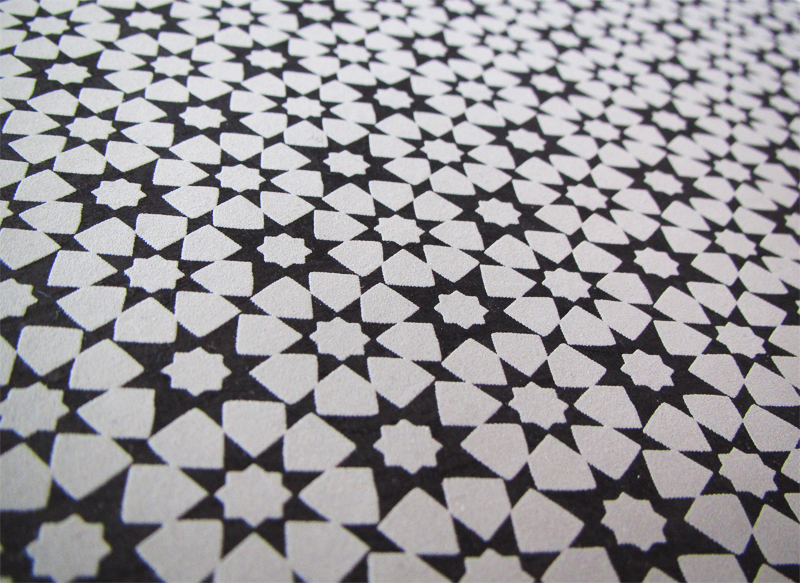
\includegraphics[height=2.5cm]{img-10/mosaico}
		
		Mosaic
		
		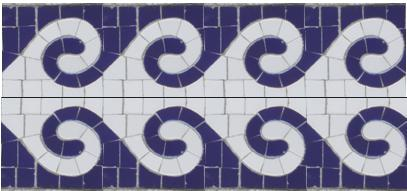
\includegraphics[height=2.5cm]{img-10/friso}
		
		Fris
		
		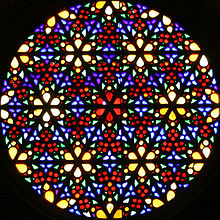
\includegraphics[height=2.5cm]{img-10/roseto}
		
		Rosetó
	\end{multicols}
	
	
\end{theorybox}

 

\begin{mylist}
	
	\vspace{-1.5cm}
	\exer \begin{minipage}[t]{0.5\textwidth}
		Observa el fris de l'imatge. És una figura que es repeteix per translació. Quina direcció té el vector de translació? D'on a on aniria?
	\end{minipage}
	\begin{minipage}{0.5\textwidth}
		\centering
		\vspace{1.5cm}
		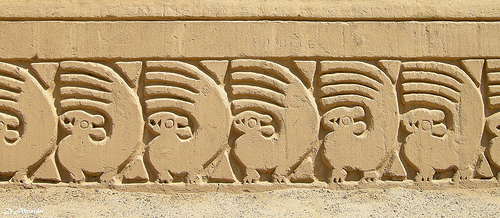
\includegraphics[width=0.7\textwidth]{img-10/fris}
	\end{minipage}
	
	\vspace{-4.5cm}
	\exer \begin{minipage}[t]{0.55\textwidth}
		En la façana d'aquesta torre mudèjar de Terol podem veure diferents translacions. En la part superior hi ha dos conjunts de quatre finestretes. Un és traslladat de l'altre. I cada finestreta forma a les altres quatre mitjançant una translació. Si seguim baixant, els dos arcs es traslladen formant altres dos arcs. Observa, en aquest cas totes les translacions tenen un vector de translació horitzontal. Continua descrivint les translacions que veus en el disseny d'aquesta torre.
	\end{minipage}
	\begin{minipage}{0.45\textwidth}
		\centering
		\vspace{4.5cm}
		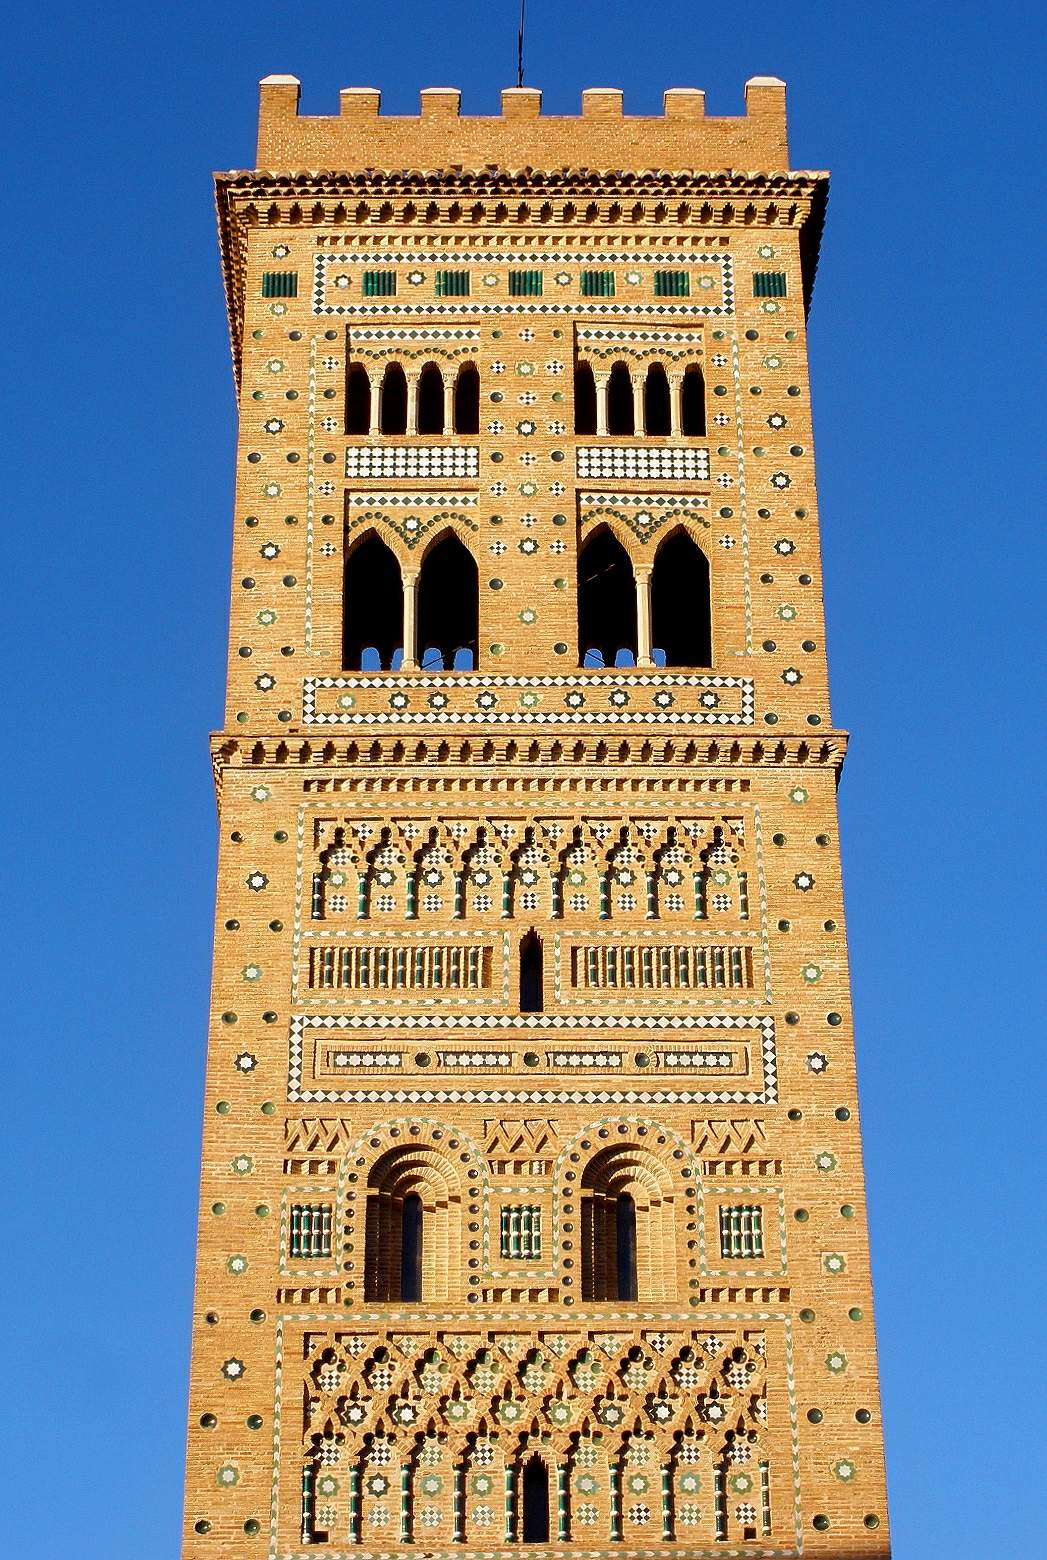
\includegraphics[width=0.4\textwidth]{img-10/mudejar}
	\end{minipage}

	\vspace{-2.5cm}
	\exer \begin{minipage}[t]{0.7\textwidth}
		El mosaic del marge està confeccionat utilitzant un motiu mínim que es desplaça per tot el mosaic. Si utilitzes com a motiu mínim l'estel de sis puntes,  determina els vectors de translació de dues translacions, una horitzontal i una altra vertical, que mitjançant composicions et permetin tenir la resta del mosaic. Observa que en sumar la translació horitzontal amb la vertical obtens translacions obliqües. Dibuixa en el teu quadern una figura i trasllada-la de forma similar per obtenir un mosaic.
	\end{minipage}
	\begin{minipage}{0.24\textwidth}
		\centering
		\vspace{2.5cm}
		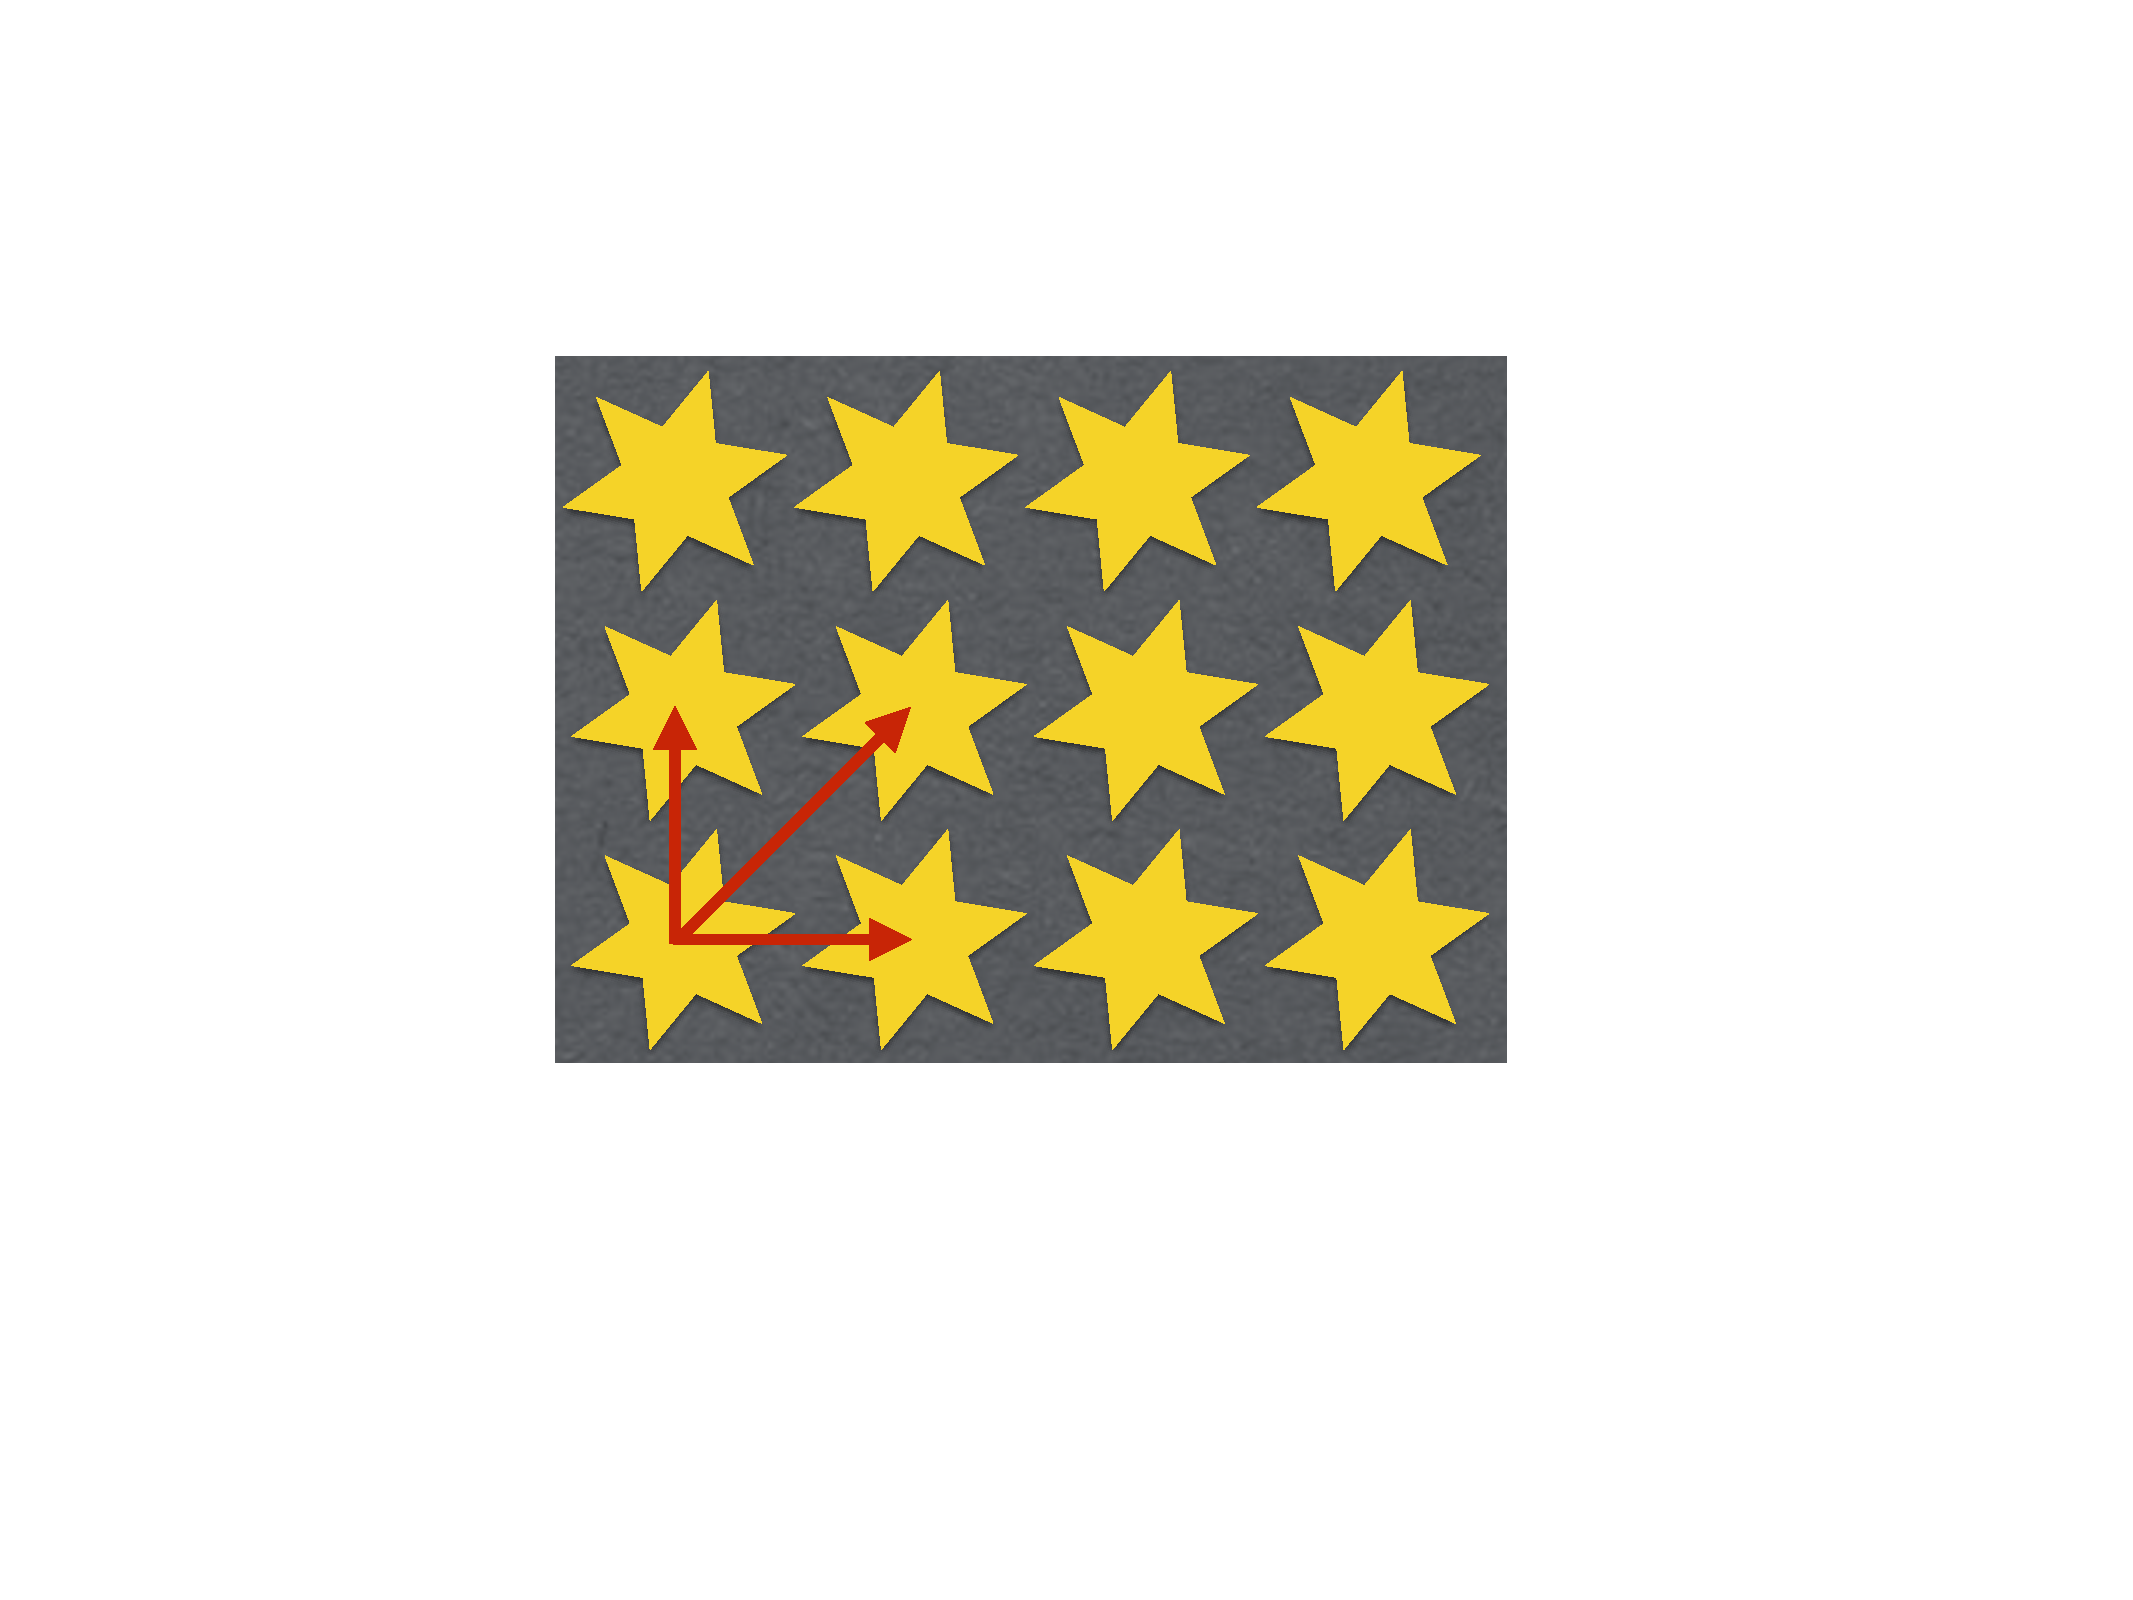
\includegraphics[width=0.9\textwidth]{img-10/mosaic}
	\end{minipage}
	
	
	
	\exer  En edificació s'utilitzen molt les translacions. Pensa en les finestres d'un edifici i tria una. Pots obtenir una altra diferent mitjançant translació? Fes un dibuix que representi aquesta situació.
	
	
	
	
\end{mylist}


\begin{mylist}
 
\exer \spen Completa el següent mosaic, fris i rosetó:
\begin{center}
	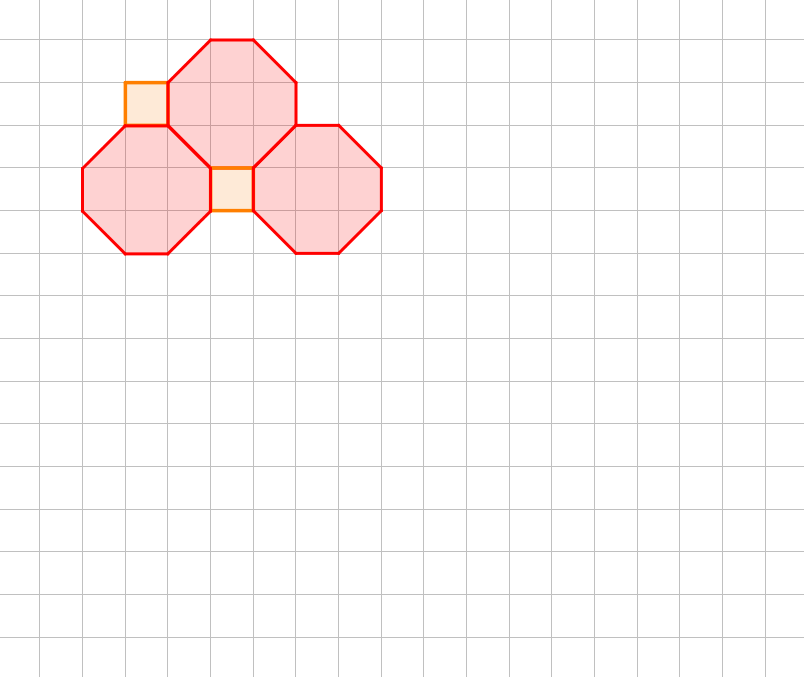
\includegraphics[height=4cm]{img-10/completa1}
	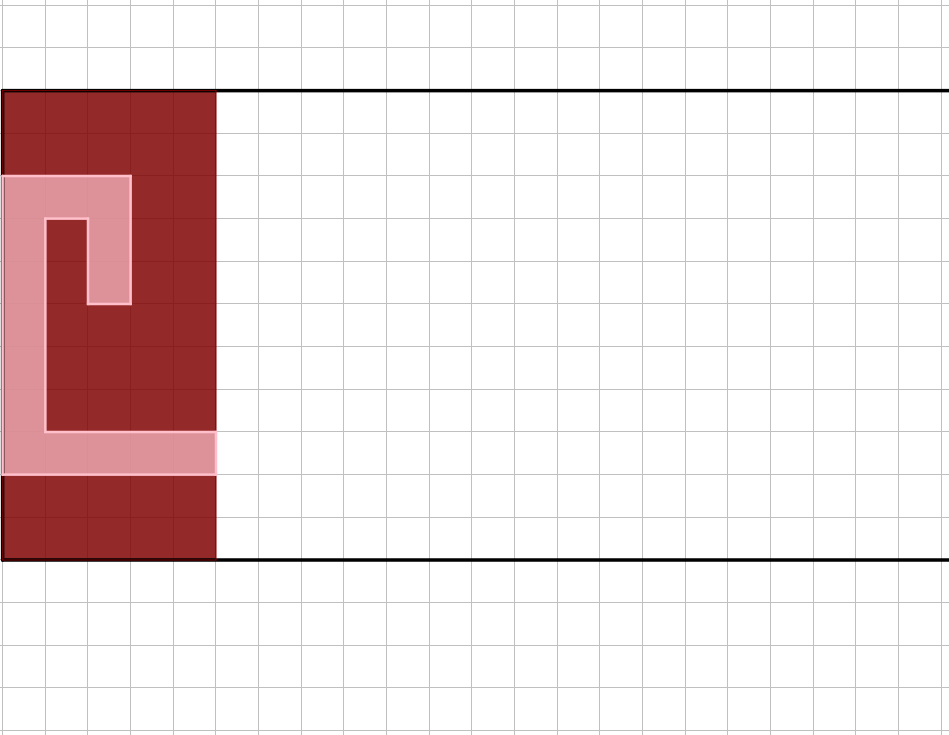
\includegraphics[height=4cm]{img-10/completa2}
	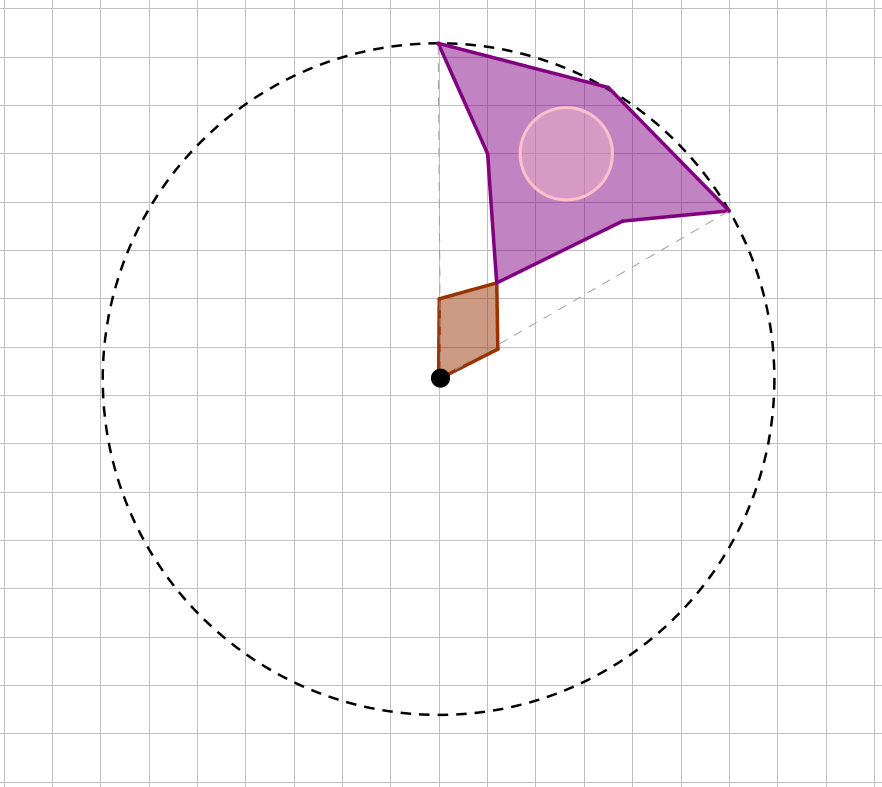
\includegraphics[height=4cm]{img-10/completa3}
\end{center}
	
\exer  Les puntes es dissenyen a partir d'un motiu que s'ha anat traslladant a tot el llarg. Dibuixa en el teu quadern un motiu, una flor, una V, un zig-zag{\dots} i trasllada-ho component diverses translacions d'un mateix vector de translació. Has dibuixat un fris.

 
\exer  Utilitza una trama de triangles, o dibuixa una en el teu quadern, per dissenyar un mosaic semblant a l'anterior. Marca en la trama els centres de girs de 60º, de 180º i de 30º. Dibuixa un motiu mínim senzill, per exemple una poligonal o una fulla, i mou-lo usant aquestes transformacions.

	\exer   Generació d'un mosaic mitjançant girs i translacions. Observa com primer dibuixa una trama de quadrats, dibuixa un motiu mínim format per dos segments, després li aplica isometries a aquest motiu: girs de 90º, amb els quals dibuixa l'estel, que per simetria completa la cel·la unitat a la qual finalment la trasllada per tot el mosaic. 
	
	
	
	\exer  Utilitza una trama de quadrats, o dibuixa una en el teu quadern per dissenyar un mosaic. Marca en la trama els centres de girs de 90º i de 180º. Marca els eixos de simetria. Dibuixa un motiu mínim senzill, per exemple una poligonal, i mou-lo usant aquestes transformacions. Completa primer la cel·la unitat, i després trasllada-la.
	
	\vspace{-1.5cm}
	\exer \begin{minipage}[t]{0.65\textwidth}
		 \textbf{Anàlisi de mosaics de l'Alhambra}: Observa el mosaic del marge. Imagina que és infinit, que completa tot el pla. Pots prendre com a motiu mínim un parell de fulletes. Per passar d'un parell de fulletes a l'altre parell adjacent, quina transformació has utilitzat? És una simetria? És un gir? Hi ha centres de gir de 60º? I d'180º? I de 30º? 
	\end{minipage}
	\begin{minipage}{0.3\textwidth}
		\centering
		\vspace{1.5cm}
		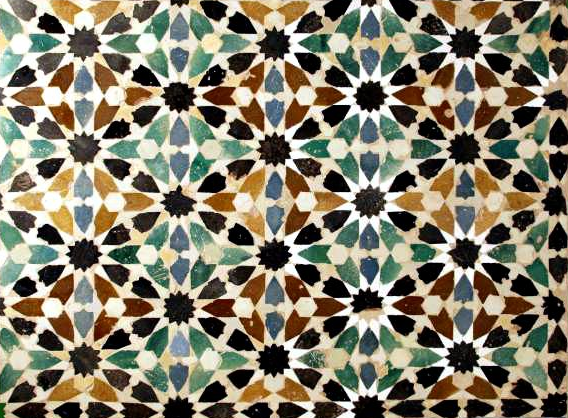
\includegraphics[width=0.85\textwidth]{img-10/granada}
	\end{minipage}

	\answers{Respecte l'estrella \textbf{*}, les fulles s'obtenen per simetria central. També \textbf{*} és el centre de gir de les fulles negres d'amplitud 180$^\circ$. Si no tenim en compte el color de les fulles, també tenim simetria de gir d'amplitud $360/12=30^\circ$}


\exer  Hem format frisos utilitzant les lletres de l'alfabet. Tots ells es formen per translació. Però en ocasions hi ha altres isometries.

\begin{tasks}(4)
\task[L1. ] \quad LLLLL
\task[L2. ] \quad NNNNN
\task[L3. ] \quad VVVVV
\task[L4. ] \quad CCCCC
\task[L5. ] \quad HHHHH
\task[L6. ] \quad pbpbpb
\task[L7. ] \quad Pqdbpqdbp
\end{tasks}

\begin{tasks}
	\task  En quins hi ha una simetria d'eix horitzontal?  I d'eix vertical?     
	\task  En quins hi ha girs de 180º.   
	\task  Hi ha simetries amb lliscament?
	\task  Assenyala totes les famílies de simetries respecte a un eix, de girs i de translacions per les quals un punt del fris es transforma en un altre punt del mateix (suposat que es perllongui fins a l'infinit).
\end{tasks}

\answers[cols=1]{[ En L4 i L5, L2 i L5, L3; L5 i L7, Sí; en L6 i L7, Translació; simetria horitzontal; simetria vertical;
	gir de 180$^\circ$  i simetria amb lliscament.]}


\exer \simbolsearch Surt al carrer o a casa teva i busca frisos. Fotografia reixes, puntes i greques{\dots} i fes un estudi dels diferents frisos que trobis. Dibuixa en el teu quadern el seu disseny i intenta classificar-los segons l'esquema de les lletres del problema anterior, segons les transformacions que utilitzin. Per a això fes-te les següents preguntes:

\begin{tasks}
\task Té girs? Si la resposta és NO, llavors:
%
\task Té simetria horitzontal? Si la resposta és SI, és un L4, que com el fris format per la lletra C o la lletra D, no té girs i si té simetria d'eix horitzontal. Si la resposta és NO, llavors:
%
\task Té simetria vertical? Si la resposta és SI, és un L3, com el fris format per la lletra V o la lletra A, que no té ni girs, ni simetria horitzontal i si té simetria vertical. Si la resposta és NO, llavors:
%
\task Té simetria amb lliscament? Si té és un L6, i si no és un L1. Però si té girs pot tenir també simetria horitzontal i és un L5, o tenir simetria amb lliscament i ser un L7, o només tenir el gir i ser un L2, com el fris format per la lletra N o la lletra S. 
 \end{tasks}


\exer  En els frisos de la dreta assenyala totes les famílies de simetries respecte a un eix, de girs i de translacions per les quals un punt del fris es transforma en un altre punt del mateix (suposat que es perllongui fins a l'infinit).

a) 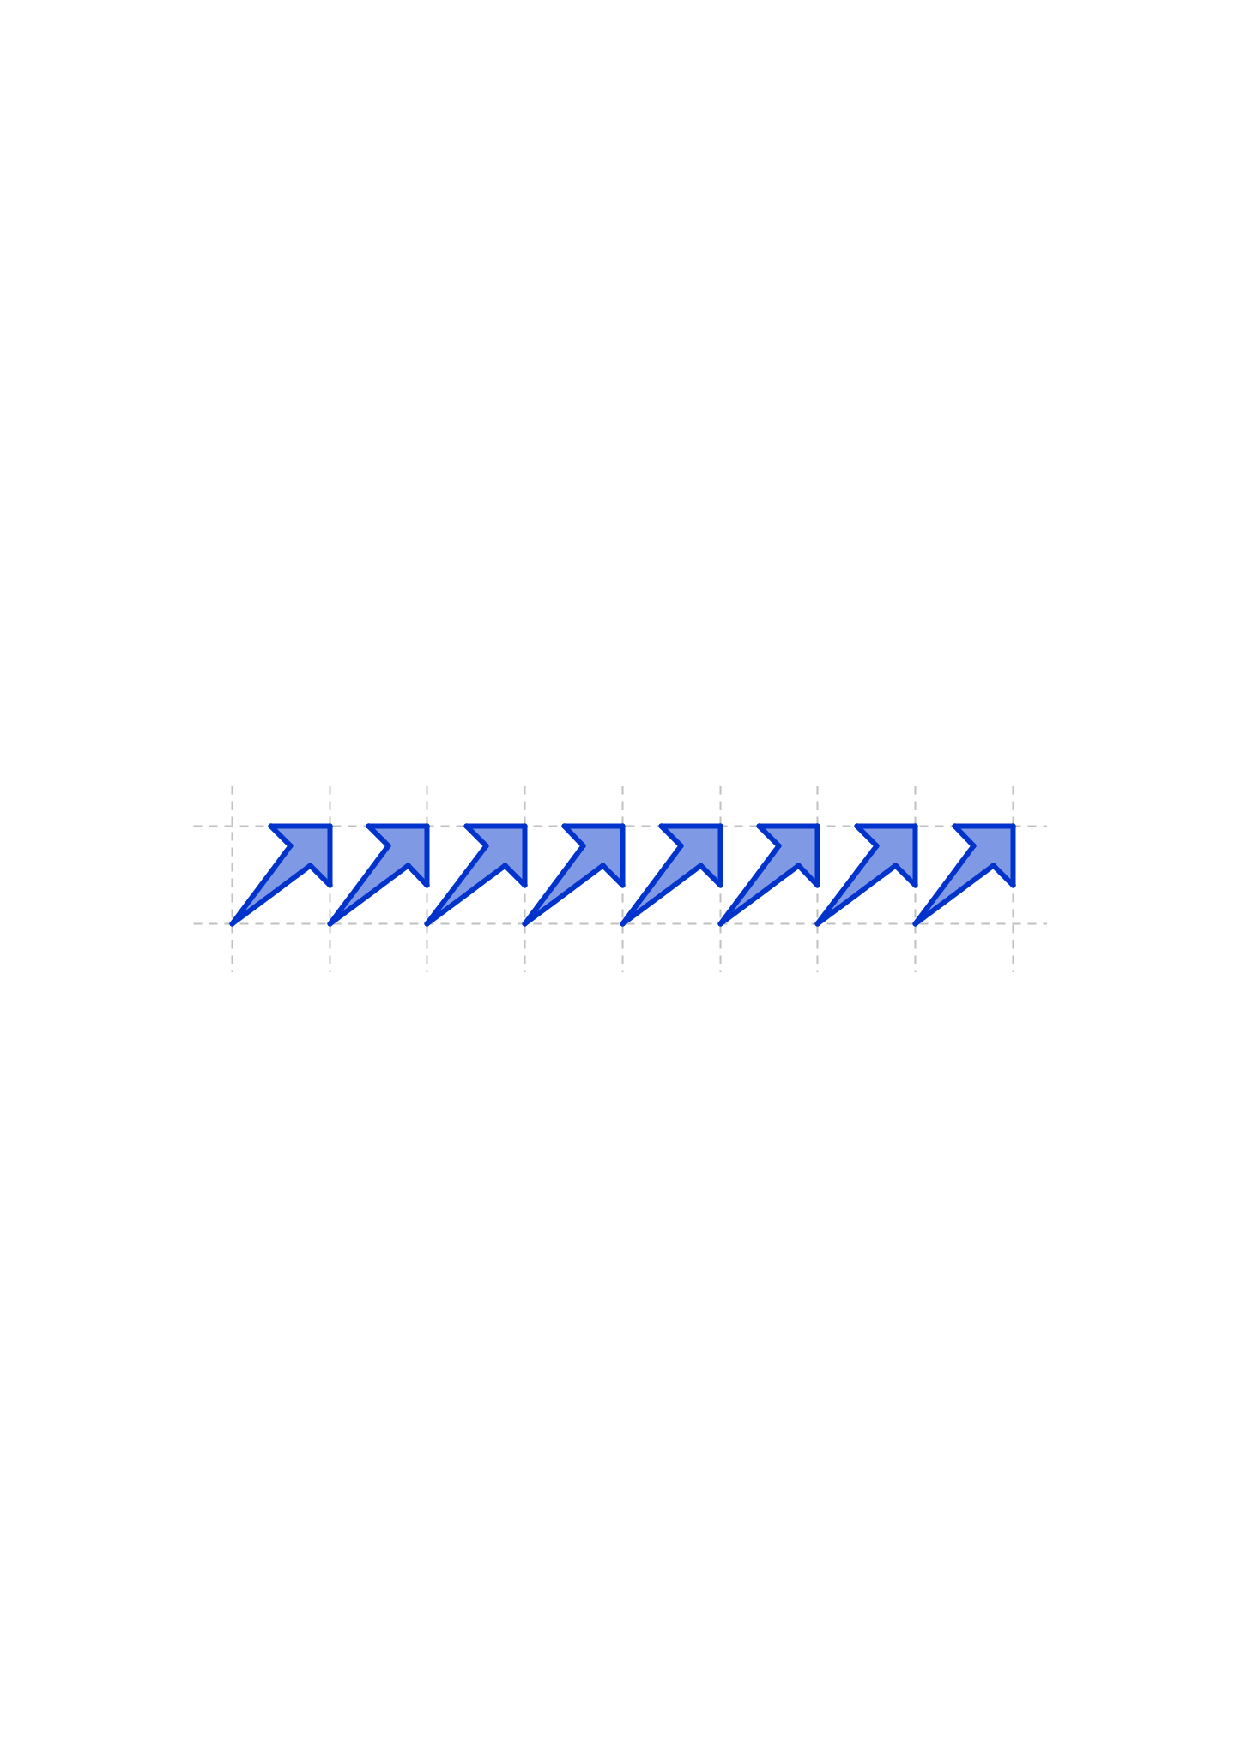
\includegraphics[height=1.2cm]{img-10/fr1}
 b)   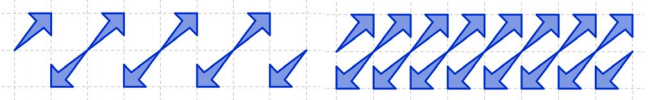
\includegraphics[height=1.2cm]{img-10/fr2}
 c)   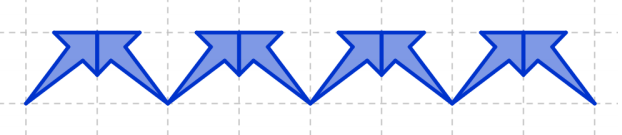
\includegraphics[height=1.2cm]{img-10/fr3}
 d) 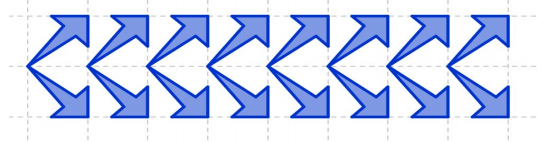
\includegraphics[height=1.2cm]{img-10/fr4}
  e)  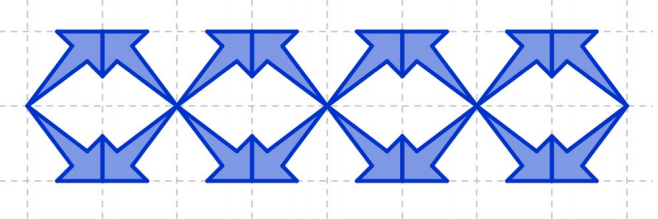
\includegraphics[height=1.2cm]{img-10/fr5}
 % f)  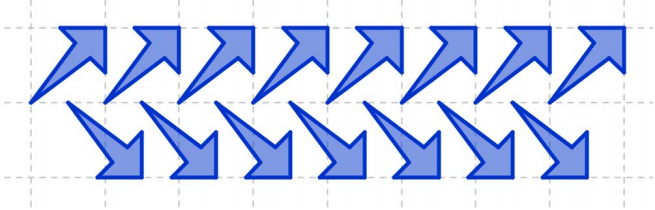
\includegraphics[height=1.2cm]{img-10/fr6}


\answers{En aquests frisos s'han utilitzat: 
	Translació, simetria horitzontal, simetria vertical, gir de 180$^\circ$, i
	simetria amb lliscament.\par 
	a) en el primer únicament hi ha translació \par
	b) girs de 180$^\circ$; \par
	c) simetria d'eix vertical\par
	d) Simetria d'eix horitzontal \par
	e)  simetries d'eix horitzontal i d'eix vertical, i per tant
	girs de 180$^\circ$}

\exer \simbolsearch \textbf{Anàlisi de tapaboques:} 

\begin{minipage}{0.4\textwidth}
	\begin{center}
		\centering
		\begin{tabular}{p{1in} p{1in}}
			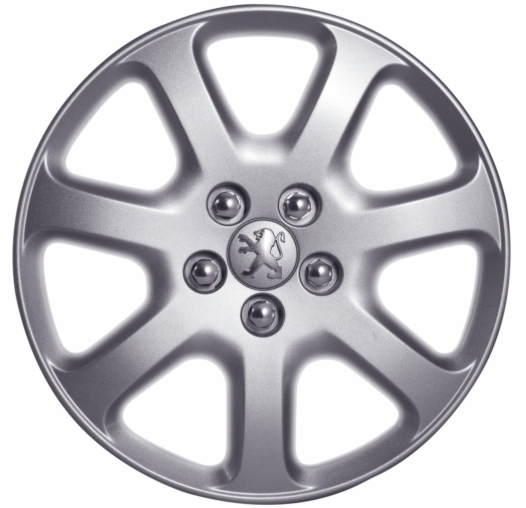
\includegraphics[height=1.2in]{img-10/tapacubos1}\par 1 &
			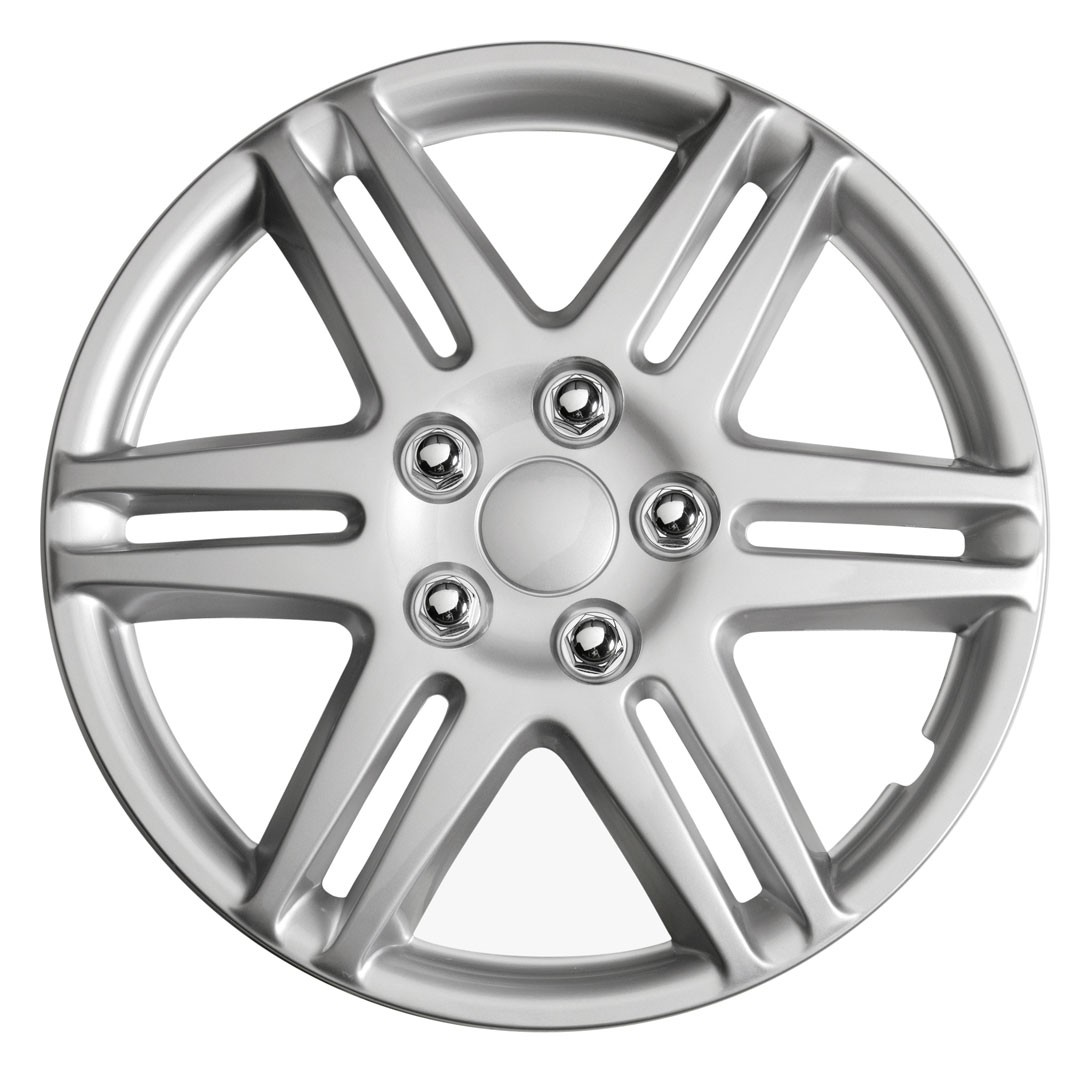
\includegraphics[height=1.2in]{img-10/tapacubos2}\par 2 \\
			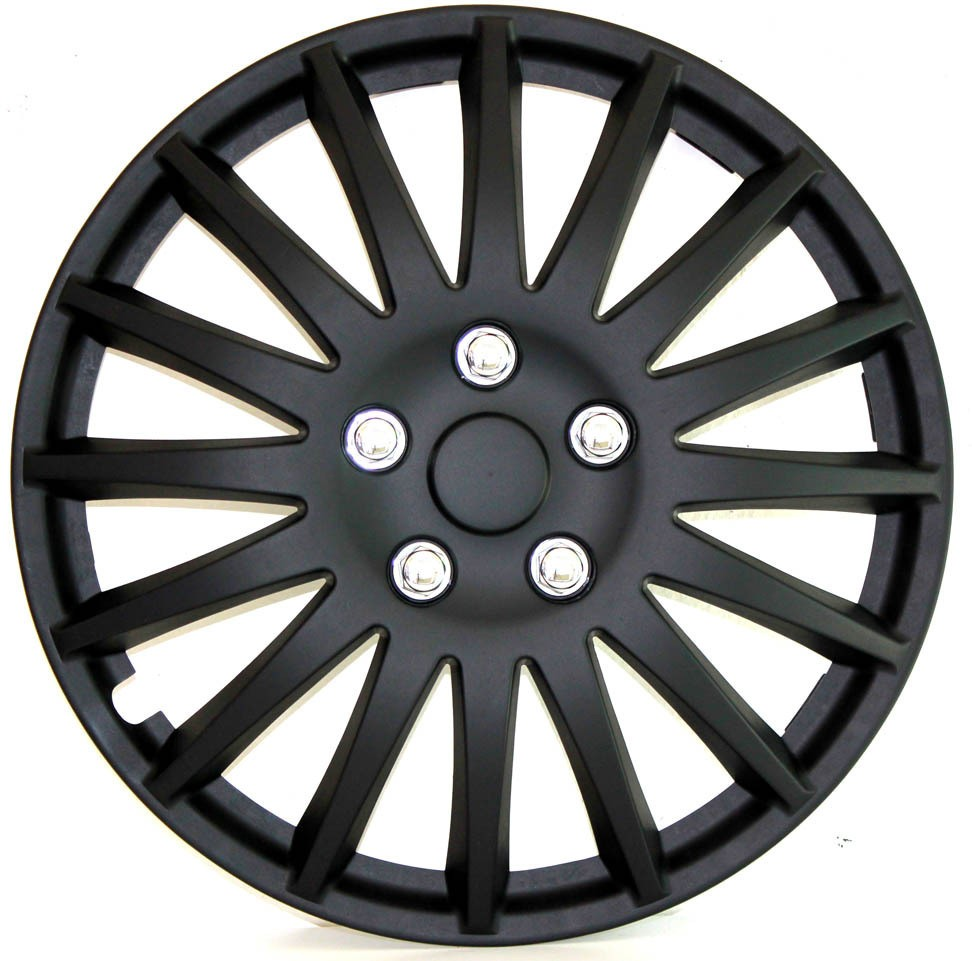
\includegraphics[height=1.2in]{img-10/tapacubos3}\par 3 &
			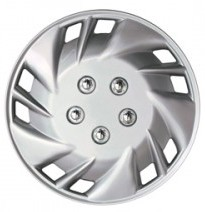
\includegraphics[height=1.2in]{img-10/tapacubos4}\par 4 \\
			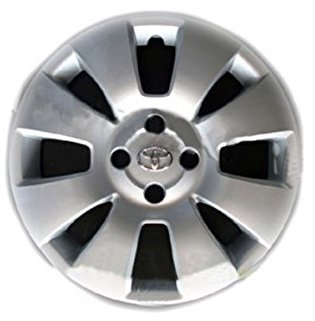
\includegraphics[height=1.2in]{img-10/tapacubos5}\par 5 &
			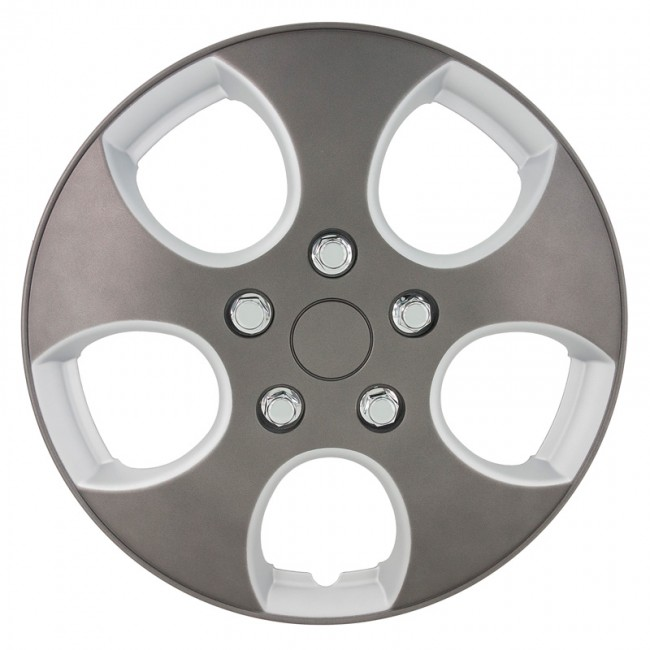
\includegraphics[height=1.2in]{img-10/tapacubos6}\par 6 \\
		\end{tabular}
	\end{center}
\end{minipage}
\begin{minipage}{0.5\textwidth}
	
	Observa els següents tapaboques. Indica, per a cadascun d'ells, les següents qüestions: 
	\vspace{0.25cm}
	
	\begin{tasks}
		\task Té simetria central?
		
		\task Té eixos de simetria axial. Quants?
		
		\task Té centre de gir, quin és el menor angle de gir que ho deixa invariant?
		
		\task Surt al carrer i fotografia o dibuixa els tapaboques que vegis i et semblin interessants. Fes un estudi d'ells.
		
	\end{tasks}

\answers[cols=1]{[Té simetria central 2; 3 i 5, Tenen simetria axial tots excepte el 4., Tots tenen centre de gir, Solució oberta]}
\end{minipage}

\begin{comment}
\begin{longtable}{|p{0.8in}|p{0.8in}|p{0.8in}|p{0.8in}|p{0.8in}|p{0.8in}|} \hline 
	\centering
	\includegraphics[width=0.8in]{img-10/image590}\par 1 &
	\includegraphics[width=0.8in]{img-10/image591}\par 2 &
	\includegraphics[width=0.8in]{img-10/image592}\par 3 &
	\includegraphics[width=0.8in]{img-10/image593}\par 4 &
	\includegraphics[width=0.8in]{img-10/image594}\par 5 &
	\includegraphics[width=0.8in]{img-10/image595}\par 6 \\ \hline
	
	\includegraphics[width=0.8in]{img-10/image596}\par 7 &
	\includegraphics[width=0.8in]{img-10/image597}\par 8 &
	\includegraphics[width=0.8in]{img-10/image598}\par 9 &
	\includegraphics[width=0.8in]{img-10/image599}\par 10 &
	\includegraphics[width=0.8in]{img-10/image600}\par 11 &
	\includegraphics[width=0.8in]{img-10/image601}\par 12 \\ \hline
	
\end{longtable}

\begin{tasks}
   \task Té simetria central?
   \task Té eixos de simetria axial. Quants?
   \task Té centre de gir, quin és el menor angle de gir que ho deixa invariant?
   \task Surt al carrer i fotografia o dibuixa els tapaboques que vegis i et semblin interessants. Fes un estudi d'ells.
\end{tasks}
\end{comment}


\end{mylist}


\begin{comment}
 
\begin{activitats}

\subsection{Translació}

\begin{mylist}
\exer  Dibuixa en el teu quadern un paral·lelogram sobre un sistema de referència i una quadrícula. Tens quatre segments orientats. Determina les coordenades dels vectors sobre aquests segments. Quins tenen les mateixes coordenades?

\exer  Dibuixa en el teu quadern un paral·lelogram sobre un sistema de referència i una quadrícula. Tens quatre segments orientats. Determina les coordenades dels vectors sobre aquests segments. Quins tenen les mateixes coordenades?

\exer  Tenim els punts \textit{A} (0, 5), \textit{B} (3, 6), \textit{C} (4, -2) i \textit{D} (7, 3). Calcula les coordenades dels vectors $\overrightarrow{AB}$; \textbf{\textit{AC}}; \textbf{\textit{AD}}; $\overrightarrow{BC}$; \textbf{\textit{BD}}; \textbf{\textit{CD}}; \textbf{\textit{DC}}; \textbf{\textit{BA}}. 

\exer  Determina el vector de translació que trasllada el punt \textit{A} (3, 7) al punt \textit{A'} (1, 5).

\exer  Per la translació de vector $\vec u$ = (2, 8) es trasllada el punt \textit{A} (9, 4) al punt \textit{A'}. Quins són les coordenades de A' ?

\exer  Per la translació de vector $\vec u$ = ($-$3, $-$1) es trasllada el punt \textit{A} a el punt \textit{A'} (3, 3). Quins són les coordenades de  A ?

\exer  Traslladem la circumferència de centre \textit{C} (5, 2) i radio 3 unitats amb la translació de vector $\vec u$ = ($-$5, $-$2). Determina el centre i el radi de la circumferència traslladada.

\exer  Dibuixa en el teu quadern uns eixos de coordenades i en ells un quadrat de costat 2 unitats al que anomenes \textit{C}, li apliques una translació segons el vector $\vec u$ = (4, 1) i anomenes \textit{C'} al seu traslladat. Ara apliques a \textit{C'} una translació segons el vector $\vec v$~=~($-$2, 4). La isometria que transforma \textit{C} en \textit{C''}, és una translació? Escriu les coordenades del seu vector. Mitjançant aquesta translació, en quin punt es transforma l'origen de coordenades?

\exer  El vèrtex inferior esquerre d'un quadrat és A (3, 1) i el vèrtex superior esquerre és B (1, 3). Li apliques una translació de vector $\vec u$ = ($-$2, 4), quins són les coordenades dels quatre vèrtexs del quadrat transformat?

\exer  Dibuixa la imatge que resulta d'aplicar al trapezi de la figura la translació de vector \textbf{\textit{OA}}~=~($-$1,~2). Determina les coordenades dels punts transformats de  A$-$( 1, 2), \textit{B} (1, 1), \textit{C}~(4,~2) i \textit{D} (5, 4) per aquesta translació. 

\begin{center}
	\includegraphics[width=0.35\textwidth]{img-10/ex1}
\end{center}

\exer  Aplica la translació de vector $\vec u$ = ($-$3, 4) al triangle \textit{ABC} de vèrtexs \textit{A} (3, 1), \textit{B }(4, 4), \textit{C} (6, 5), i calcula les coordenades del triangle transformat.

\exer  Dibuixa en el teu quadern un cercle de centre l'origen i radi 2 unitats. 

\begin{tasks}
	\task  Trasllada-ho amb la translació de vector $\vec u$ = (3, 0).
	\task  Trasllada-ho després mitjançant la translació de vector $\vec v$ = (0, 4).
	\task  Indica les coordenades del centre del segon cercle traslladat.
	\task  Indica les coordenades del traslladat del punt (0, 2) en aplicar-li cadascuna de les dues translacions.
\end{tasks}


\exer  Traslladem el triangle \textit{ABC} de vèrtexs \textit{A} (6, 1), \textit{B} ($-$3, 4) i \textit{C} (0, 8), mitjançant la translació de vector $\vec u$ = (7, 1), i després mitjançant la translació de vector $\vec v$ = (2, 8). Determina les coordenades del triangle transformat analítica i gràficament.

\exer  La composició de dues translacions té per vector (5, 9). Si una d'elles és la translació de vector $\vec u$ = (7, 3), quins components té l'altre vector de translació?

\exer  a) Dibuixa en el teu quadern un triangle \textit{ABC} i trasllada-ho 5 cm a la dreta. Denomina \textit{A'B'C'}${}_{ }$al triangle obtingut.

\exer  Trasllada \textit{A'B'C'} ara 4 cm cap amunt i denomina \textit{A''B''C''} al nou triangle. 

\exer  Dibuixa el vector que permet passar directament del triangle \textit{ABC} a l'A''B''C''  i mesura la seva longitud. Quines són les seves coordenades?

\exer  Determina el vector de translació de la translació inversa a la de vector $\vec u$ = ($-$2, 5).

\exer  a) Dibuixa en el teu quadern una figura, i repeteix el dibuix traslladant la figura 4 vegades amb la mateixa translació. En fer-ho, dibuixaràs un fris. 

\exer  Un fris confeccionat amb lletres L és: L L L L L. Dibuixa un fris confeccionat amb lletres J. Un altre confeccionat amb lletres M. A més de translació, té simetries?

\exer  Busca un fris. Mira les reixes del teu carrer, un brodat o una punta, les greques d'uns taulells{\dots} i dibuixa el seu disseny en el teu quadern.

\exer  Mitjançant una translació en l'espai, en què es transforma un pla? I una esfera? I un con? I dos plans paral·lels? I dos plans ortogonals? Analitza els resultats.

\end{mylist}
 


\subsection{Girs}

\begin{mylist}
\exer  Dibuixa en el teu quadern el punt \textit{A} (5, 4). Indica les coordenades del punt \textit{A' }que s'obté en girar 180º i amb centre l'origen el punt \textit{A}. Indica les coordenades del punt \textit{A''} obtingut en girar \textit{A'   }90º amb el mateix centre de gir.

\exer  Dibuixa una figura en el teu quadern, calca-la, retalla-la i pega-la inclinada al costat de la inicial. Les dues figures, tenen totes les longituds iguals?, i els seus angles? Determina, amb compàs i transportador, el centre i l'angle de gir.

\exer  Dibuixa en el teu quadern una lletra F i la lletra F girada 30º amb centre de gir el seu punt més inferior.

\exer  Dibuixa en el teu quadern un triangle rectangle isòsceles i amb centre en el vèrtex d'un dels angles aguts aplica-li un gir de 45º en sentit positiu. Després aplica-li un altre gir de 45º, i així successivament fins a arribar al triangle inicial. Quins girs has estat fent?

\exer  Dibuixa en el teu quadern un cercle de centre \textit{O}, dos diàmetres perpendiculars \textit{AB}  \textit{i CD} i una corda \textit{CB}. Sobre el mateix dibuix traça les figures obtingudes fent girar la figura formada pels dos diàmetres i la corda, amb girs de centre \textit{O} i angles 45º, 90º, 135º, 180º, 225º, 270º i 315º. Hauràs fet la composició de girs de 45º diverses vegades.

\exer  La lletra H té centre de simetria? Indica tres objectes quotidians que tinguin simetria central.

\exer  Sobre uns eixos cartesians representa els punts \textit{A} (2, 6), \textit{B} ($-$2, 5), \textit{C} (5, 3) i els seus simètrics respecte a l'origen \textit{A', B'} i \textit{C'}. Quines coordenades tenen \textit{A'}, \textit{B'} i \textit{C'}?

\exer  Dibuixa en el teu quadern el triangle de vèrtexs \textit{A} (3, 7), \textit{B} (5, $-$5) i \textit{C} (7, 2). Dibuixa el triangle que s'obté en girar-lo amb centre en el punt \textit{D} (8, 8) un angle de 180º. És una simetria central. Quines són les coordenades dels vèrtexs \textit{A'}, \textit{B'} i \textit{C'} del nou triangle?

\exer  Dibuixa en un sistema de referència un punt  P i el seu simètric \textit{P'} respecte de l'origen. Si les coordenades de P són (\textit{x},~y), quines són les de \textit{P'}?

\exer  Donat el triangle \textit{A}( 3, $-$4), \textit{B} (5, 6), \textit{C} ($-$4, 5), troba les coordenades dels vèrtexs del triangle simètric respecte de l'origen.

\exer  Dibuixa un triangle equilàter \textit{ABC} i amb centre en el vèrtex \textit{A} aplica-li un gir d'angle 60º. El triangle donat i el transformat, quina figura formen? Torna a aplicar al triangle transformat el mateix gir de centre \textit{A}, quins girs has estat fent? Quants girs has d'aplicar al triangle inicial perquè torni a ocupar la posició inicial?

\exer  Dibuixa en el teu quadern els quatre punts de la figura. Determina, amb regla, compàs i transportador, el centre i l'angle de gir sabent que els punts \textit{A}  \textit{i B} s'han transformat mitjançant un gir en \textit{A'} i \textit{B'}.

\begin{center}
	\includegraphics[width=0.3\textwidth]{img-10/ex2}
\end{center}


\exer  Dibuixa la imatge que resulta d'aplicar al triangle de la figura el gir de centre \textit{O} que transforma el punt \textit{A} en el punt \textit{B}. 


\begin{center}
	\includegraphics[width=0.3\textwidth]{img-10/ex3}
\end{center}

\exer  Utilitza un transportador d'angles, regla i compàs, per girar una recta 60º respecte a un punt \textit{O} exterior a ella (és suficient girar dos punts d'aquesta recta). Mesura els angles que formen les dues rectes, la inicial i la girada. Observes alguna regularitat? Investiga un mètode per girar una recta transformant un sol punt. Quin punt has de triar i per què? 

\exer   \textbf{Joc per a dos jugadors}: Forma sobre la taula un polígon regular utilitzant monedes (o fitxes o boletes de paper) com a vèrtexs. Alternativament cada jugador retira o una moneda o dues monedes adjacents. Guanya qui retiri l'última moneda. (\textbf{\textit{Ajuda}}: És un joc d'estratègia guanyadora que pots descobrir utilitzant la simetria central). 

 
\exer  En el disseny d'aquest mosaic s'han utilitzat girs en el pla. No ho veiem complet, però podem imaginar que fos infinit. Indica els centres de gir que vegis. En el centre de la figura hi ha un centre de gir claríssim, de quin angle? Hi ha girs de 45º? Quins són els seus centres de gir? Hi ha centres de simetria? Indica'ls. 
 

\exer  Per a cadascun dels següents polígons indica el centre de gir i el mínim angle de gir que deixen invariants a cadascun d'ells:

\begin{tasks}
	\task  Pentàgon regular   
	\task  Hexàgon regular    
	\task  Decàgon regular
	\task  Triangle equilàter   
	\task  Rectangle    
	\task  Quadrat
	\task  Rombe     
	\task  Paral·lelepípede   
	\task  Octògon regular
\end{tasks}



\exer  Indica si el mosaic de l'Alhambra de sota té centre de gir, i determina quin és el menor angle de gir que fa que el mosaic se superposi (sense tenir en compte els canvis de color). Hi ha centres de simetria?

\begin{center}
	\includegraphics[width=3cm]{img-10/image606}
\end{center}

\exer  Amb ajuda de paper quadriculat transforma mitjançant una simetria central, una recta, una circumferència, un segment, un triangle, dues rectes paral·leles i dues rectes perpendiculars. En què es transformen? Analitza els resultats.

\exer  Quin nombre mínim de quadrats és necessari pintar de verd perquè el quadrat gran de l'esquerra tingui un centre de simetria?

\begin{center}
	\includegraphics[width=0.15\textwidth]{img-10/quadradets}
\end{center}

\exer  Hem girat el punt \textit{A} (3, 5) i hem obtingut el punt \textit{A'} (7, $-$2). Determina el centre de gir i l'angle utilitzant regla, compàs i transportador d'angles.

\exer  Quins dels polígons estrellats de la figura de sota tenen centre de simetria? Indica el centre de gir i el mínim angle de gir que deixa invariants a cadascun d'ells. 

\begin{center}
	\includegraphics[width=0.4\textwidth]{img-10/estrelles}
\end{center}

\exer  Determina tres objectes quotidians que tinguin algun eix de gir.

\exer  En la simetria central de centre (2, 3) hem vist que el simètric del punt \textit{A} (8, 1) és el punt \textit{A'} ($-$4, 5). Calcula els simètrics dels punts \textit{B} (12, 7), \textit{C} (9, 10), \textit{D} (5, 8) i \textit{E }(7, 6).
 
 

\end{mylist}


\subsection{Simetries}

\begin{mylist}

\exer  Dibuixa en el teu quadern un sistema de referència i una lletra B. Dibuixa la lletra simètrica de  B respecte de l'eix d'abscisses i respecte de l'eix d'ordenades.

\exer  Classifica les lletres majúscules de l'alfabet.

\begin{tasks}
	\task  les que són simètriques respecte d'un eix de simetria horitzontal i un eix de simetria vertical.
	\task  les que només són simètriques respecte d'un eix de simetria vertical,
	\task  les que només ho són respecte de l'eix de simetria horitzontal,
	\task  les que no tenen cap eix de simetria.
	\task  Comprova que les lletres que tenen dos eixos de simetria tenen centre de simetria. La raó ja la saps: La composició de dues simetries d'eixos secants és un gir.
\end{tasks}




\exer  Quines de les següents successions de lletres tenen un únic eix de simetria? Quines tenen dos eixos? Quines cap? Quines tenen centre de simetria?

\begin{tasks}(2)
	\task  ONO  
	\task  NON 
	\task  DODO 
	\task  OIO   
	\task  HEMO  
	\task  HOOH
\end{tasks}



\exer  Indica els eixos de simetria de les següents figures: 

\begin{tasks}(2)
	\task  Quadrat   
	\task  Triangle equilàter.  
	\task  Trapezi isòsceles.  
	\task  Hexàgon.   
	\task  Circumferència.   
	\task  Rectangle.   
	\task  Rombe.    
	\task  Pentàgon.
\end{tasks}



\exer  Considera que els vèrtexs del quadrilàter de la figura tenen de coordenades: (1, 3), (2, 3), (3, 2) i (2, 4). Aplica-li dues simetries axials d'eixos  paral·lels, la primera respecte a l'eix \textit{r} i la segona respecte a l'eix \textit{s}. 

\begin{center}
	\includegraphics[width=0.3\textwidth]{img-10/axial1}
\end{center}

\begin{enumerate}
 
\exer  Indica les coordenades dels vèrtexs de les figures transformades per aquesta composició de simetries.


 Si anomenem \textit{C} al quadrilàter inicial, \textit{C'} al seu simètric respecte a l'eix \textit{r} i \textit{C''} al simètric de \textit{C'} respecte a l'eix \textit{s}:


\exer  Quina isometria ens permet transformar directament \textit{C }en \textit{C''}.

\exer  Quins elements la defineixen? 

\exer Què ocorre si apliquem les dues simetries en diferent ordre, primer respecte a l'eix \textit{s} i després respecte a l'eix \textit{r}? Quines són ara les coordenades dels vèrtexs de la figura \textit{C'''} transformada?


\end{enumerate}

 
\exer  Considera que els vèrtexs del quadrilàter de la figura tenen de coordenades: (1, 3), (2, 3), (3, 2) i (2, 4). Aplica-li dues simetries axials d'eixos secants, la primera respecte a l'eix \textit{r} i la segona respecte a l'eix \textit{s}. 

\begin{center}
	\includegraphics[width=0.35\textwidth]{img-10/axial2}
\end{center}

\begin{enumerate}
 
\exer  Indica les coordenades dels vèrtexs de les figures transformades per la composició de simetries.

\exer  Si anomenem \textit{C} al polígon inicial, \textit{C'} al simètric respecte a l'eix \textit{r} i \textit{C''} al simètric de \textit{C'} respecte a l'eix \textit{s}: Quina isometria ens permet transformar directament \textit{C} en \textit{C''}. Quins elements la defineixen? 

\exer  Què ocorre si apliquem les dues simetries en diferent ordre, primer respecte a l'eix \textit{s} i després respecte a l'eix \textit{r}? Quina isometria tenim ara? Quins elements la defineixen? 

\exer  Indica les coordenades dels vèrtexs de la figura transformada si primer apliquem la simetria d'eix \textit{s }i després la d'eix  \textit{r}.

\end{enumerate}

\exer  Dibuixa en un paper el contorn d'una figura irregular, en almenys cinc posicions. (Si no se t'ocorre cap figura, dibuixa una lletra G).

\begin{tasks}
	\task  Són iguals aquestes figures? Explica el teu raonament.
	\task  Com pots passar d'una figura a una altra?
	\task  Acoloreix amb el mateix color totes les figures que pots aconseguir des de la posició inicial, desplaçant la figura sense aixecar-la. Utilitza un altre color per a les restants.
\end{tasks}


 Es pot passar sempre d'una figura a una altra del mateix color, lliscant la figura sense donar-li la volta? Canvien les dimensions de la figura?


\exer   El triangle equilàter T de la figura s'ha transformat en el triangle T' mitjançant una simetria axial d'eix \textit{r}. a) Copia el dibuix en el teu quadern i assenyala en el dibuix a \textit{A'}, \textit{B'} i \textit{C'}, que són els transformats de A, \textit{B }i\textit{ C} respectivament. b) Troba un gir que transformi T en T', indicant el centre i l'angle de gir, quins són ara els transformats dels vèrtexs \textit{A, B i C}?

\begin{center}
	\includegraphics[width=0.35\textwidth]{img-10/axial3}
\end{center}

\exer  \textbf{Llibre de miralls:} Utilitza un llibre de miralls per obtenir simetries. Pots construir un amb dos rectangles de metacrilat units amb cinta d'embalar. Mira pel llibre de miralls un segment, una circumferència, diferents figures{\dots}

\exer \textbf{La simetria en l'escriptura de Leonardo da Vinci: } Sabies que, si mires l'escrit per Leonardo da Vinci en un mirall pots llegir-lo amb facilitat? És un bon exemple de simetria especular. Recordes algun altre cas on s'utilitza aquesta simetria?


\begin{center}
	\includegraphics[width=0.45\textwidth]{img-10/leonardo}
\end{center}
\end{mylist}

\begin{comment}

\subsection{Problemes}

\begin{mylist}
\exer  Indica els punts invariants i les rectes invariants en cadascun dels següents moviments.

\exer  \includegraphics*[bb=0 0 1.25in 1.18in, width=1.25in, height=1.18in, keepaspectratio=false]{img-10/image52.png}Una translació segons el vector (1, 3).

\exer  Una simetria axial respecte a l'eix d'ordenades.

\exer  Una simetria central respecte al centre de coordenades.

\exer  En la figura adjunta l'hexàgon 1, denominat H1, ha canviat de posició mitjançant moviments.

\begin{tasks}
	\task  Indica el tipus de moviment: translació, gir o simetria que transforma H1 en cadascun dels altres hexàgons.
	\task  Determina, en cada cas, els elements bàsics que defineixen cada transformació indicant les coordenades de cadascun dels vèrtexs d'H1 quines coordenades té en cadascun dels transformats, i si és possible, generalitza. 
\end{tasks}


\exer  Sabem que les translacions no deixen cap punt invariant, però,

\begin{tasks}
 \task  deixa alguna recta invariant?
 \task  La simetria central deixa un punt invariant, el centre, però, quines rectes deixa invariants una simetria central en el pla? I una simetria central en l'espai?
 \task  Una simetria axial deixa invariants tots els punts del seu eix, que és una recta invariant de punts invariants, però quines altres rectes invariants deixa una simetria axial? I quins altres punts?
 \task  Una simetria especular, en l'espai, deixa un pla invariant de punts invariants, el pla de simetria, quins altres pla deixa invariants? Quines altres rectes? Quins altres punts?
\end{tasks}
 

 


\exer  Copia en el teu quadern i completa les següents taules:


\begin{tabular}{|p{1.1in}|p{0.9in}|p{0.9in}|p{1.5in}|} \hline 
\textbf{Taula I: En el pla} & \textbf{Punts invariants} & \textbf{Rectes invariants} & \textbf{Rectes invariants de punts invariants} \\ \hline 
\textbf{Translació} &  &  &  \\ \hline 
\textbf{Simetria central} &  &  &  \\ \hline 
\textbf{Gir} &  &  &  \\ \hline 
\textbf{Simetria axial} &  &  &  \\ \hline 
\textbf{Simetria amb lliscament} &  &  &  \\ \hline 
\end{tabular}



\begin{tabular}{|p{1.1in}|p{1.1in}|p{1.1in}|p{1.1in}|} \hline 
\textbf{Taula II: En l'espai} & \textbf{Punts invariants} & \textbf{Rectes invariants} & \textbf{Plans invariants} \\ \hline 
\textbf{Translació} &  &  &  \\ \hline 
\textbf{Simetria central} &  &  &  \\ \hline 
\textbf{Gir} &  &  &  \\ \hline 
\textbf{Simetria especular} &  &  &  \\ \hline 
\textbf{Simetria amb lliscament} &  &  &  \\ \hline 
\end{tabular}


\exer  Dibuixa el triangle T de vèrtexs \textit{A }(2, 1), \textit{B }(4, 2) i \textit{C }(1, 3)

\exer  Aplica a T una translació segons el vector $\vec u$ = ($-$3, 2), anomena T' al seu transformat i indica les coordenades dels seus vèrtexs.

\exer  Dibuixa el triangle T'' que resulta d'aplicar a T un gir de 270º respecte a l'origen de coordenades i indica les coordenades dels seus vèrtexs.

\exer  Dibuixa el quadrat \textit{K} de vèrtexs \textit{A }(2, 1), \textit{B }(4, 2) \textit{C }(1, 3) i \textit{D }(3, 4).

\exer  Aplica a  K una translació segons el vector $\vec u$ = ($-$3, $-$1), anomena \textit{K}' al seu transformat i indica les coordenades dels seus vèrtexs.

\exer  Dibuixa el quadrat \textit{C}'' que resulta d'aplicar a   C una simetria central respecte al punt (3, 0) i indica les coordenades dels seus vèrtexs.


 
\end{mylist}
 
\end{activitats}

\end{comment}


\newpage
\begin{autoaval}{52}

\begin{mylist}
\exer[2] Amb la translació de vector $\vec u = (-3, 8)$ traslladem el punt  $P (5, -4)$ fins al punt \textit{P'} i les coordenades de \textit{P'} són:
\begin{tasks}(4)
	\task  (8, 4)    
	\task  (2, 4)    
	\task  (2, 12)   
	\task  (6, 3)
\end{tasks}
\answers{\textbf{--10. } Autoavaluació: 1b; 2c; 3b; 4d; 5c; 6b; 7b; 8b; 9d; 10b;}

\exer En traslladar \textit{A}(  $-$1, 8) fins a \textit{A'} (4, 6) s'utilitza el vector $\vec u$:
\begin{tasks}(4)
	\task  $\vec u$ = (3, 2)   
	\task  $\vec u$ = (3, $-$2)   
	\task  $\vec u$ = (5, $-$2)   
	\task  $\vec u$ = (5, 14)  
\end{tasks}

\exer La transformació que converteix el punt \textit{A} (2, 0) en el punt \textit{A'} (0, 2) \textbf{no} pot ser:
\begin{tasks}(2)
	\task  Un gir de centre l'origen i angle 90º  
	\task  Una translació de vector $\vec u$ = (2, 2)
	\task  Un gir de centre l'origen i angle 270º  
	\task  Una simetria d'eix \textit{y = x}.
\end{tasks}

\exer La transformació identitat també es diu:
\begin{tasks}(4)
	\task  Simetria central   
	\task  Simetria axial  
	\task  Gir de 180º   
	\task  Translació de vector nul (0, 0)
\end{tasks}

\exer Com ha de ser un triangle per tenir més de dos eixos de simetria?
\begin{tasks}(4)
	\task  rectangle    
	\task  isòsceles    
	\task  equilàter
	\task  rectangle isòsceles
\end{tasks}

\exer La simetria central en el pla és un gir de:
\begin{tasks}(4)
	\task  360º    
	\task  180º    
	\task  90º    
	\task  0º
\end{tasks}

\exer En el pla, la composició de dues simetries d'eixos secants sempre és:
\begin{tasks}(2)
	\task  una translació   
	\task  un gir   
	\task  una altra simetria  
	\task  la simetria central
\end{tasks}

\exer Les coordenades del punt simètric al punt \textit{A} (3, 7) respecte de l'eix d'ordenades són:
\begin{tasks}(4)
	\task  \textit{A'} ($-$3, 7)   
	\task  \textit{A'} (3, $-$7)    
	\task  \textit{A'} ($-$3, $-$7)  
	\task \textit{ A'} (7, 3)
\end{tasks}

\exer Indica quina de les següents lletres \textbf{no }té simetria central:
\begin{tasks}(4)
	\task  O     
	\task  H    
	\task  S   
	\task  D
\end{tasks}

\exer Sempre s'obté un gir fent successivament:
\begin{tasks}(2)
	\task  Dos girs de diferent centre   
	\task  Dues simetries d'eixos secants
	\task  Un gir i una simetria    
	\task  Dues simetries d'eixos paral·lels.
\end{tasks}

\end{mylist}
\end{autoaval}

\newpage
\resum
\begin{center}
	\renewcommand{\arraystretch}{1.8}
\begin{longtable}{|p{0.2\textwidth}|p{0.36\textwidth}|p{0.36\textwidth}|} \hline 
	
\cellcolor{lightgray} \textbf{Homotècia} & Transformació geomètrica  que conserva els angles i les distàncies són proporcionals. & Un fotocopia reduïda \\ \hline 

\cellcolor{lightgray} \textbf{Translació} & Ve determinada pel seu vector de translació.\newline Són isometries directes.\newline La composició de dues translacions és una translació. & El traslladat del punt P (1, 2) per la translació de vector $\vec v$ = (4, 5) és P'~(5,~7). \\ \hline 

\cellcolor{lightgray} \textbf{Gir o rotació en el pla}\newline\textbf{ Gir en l'espai} & Ve determinat pel centre de gir i l'angle de gir.\newline Ve determinat per l'eix de gir i l'angle & El girat del punt P (1, 2) pel gir de centre l'origen i angle 90º és \newline P' ( 2, $-$1) \\ \hline 

\cellcolor{lightgray} \textbf{Simetria axial}\newline \textbf{Simetria especular} & Es coneix pel seu eix de simetria\newline Es coneix pel seu pla de simetria & El simètric del punt P (1, 2) per la simetria d'eix l'eix d'ordenades és P'~($-$1,~2) \\ \hline 

\cellcolor{lightgray} \textbf{ Isometries} & Són transformacions geomètriques que conserven les distàncies i els angles. & Translacions, girs i simetries \\ \hline 

\cellcolor{lightgray} \textbf{Composició d'isometries}  & \multicolumn{2}{|p{0.74\textwidth}|}{La composició de dues isometries directes és una isometria directa.\newline La composició de dues isometries inverses és una isometria directa.\newline La composició d'una isometria directa amb una inversa és una isometria inversa.} \\ \hline 

\cellcolor{lightgray} \textbf{Composició d'isometries en el pla} & \multicolumn{2}{|p{0.74\textwidth}|}{La composició de dos girs del mateix centre és un gir del mateix centre.\newline La composició de dues simetries és un gir o una translació.} \\ \hline 

\cellcolor{lightgray} \textbf{Elements invariants en el pla} & \multicolumn{2}{|p{0.74\textwidth}|}{La \textbf{translació} no deixa \textbf{cap} punt invariant.\newline El \textbf{gir} deixa invariant \textbf{un} punt, el centre de gir.\newline La \textbf{simetria} deixa invariant una \textbf{recta}, l'eix de simetria\newline La \textbf{identitat} deixa invariant \textbf{tot} el pla.}   \\ \hline 

\cellcolor{lightgray} \textbf{Elements invariants en l'espai} & \multicolumn{2}{|p{0.74\textwidth}|}{La \textbf{translació} no deixa \textbf{cap} punt invariant.\newline La \textbf{simetria central} deixa invariant \textbf{un} únic punt, el centre de simetria.\newline El \textbf{gir} deixa invariant una \textbf{recta}, l'eix de gir.\newline La \textbf{simetria} deixa invariant el \textbf{pla} de simetria\newline La \textbf{identitat} deixa invariant \textbf{tot} l'espai.} \\ \hline 

\end{longtable}
 
\end{center}